%% ===================================================================
%% Deep Learning Latency Attacks and Defenses: A Survey
%% Target venue: ACM Computing Surveys (CSUR)
%% Document class: acmart (acmsmall = journal / CSUR format)
%% ===================================================================
\documentclass[acmsmall,screen,review,nonacm]{acmart}
%\documentclass[acmsmall,screen,nonacm]{acmart}
\setlength{\headheight}{18.48402pt}
%% --- Packages ---
\usepackage{booktabs}
\usepackage{graphicx}
\usepackage{multirow}
\usepackage{array}
\usepackage{xcolor}
\usepackage{amsmath}
\usepackage{tabularx}
\usepackage{wasysym}   % \CIRCLE \LEFTcircle \Circle harvey-ball symbols
\usepackage{pifont}    % \ding{55} cross mark
\usepackage{fontawesome5} % \faGithub \faFilePdf
\usepackage{longtable}    % page-breaking appendix catalog tables
\usepackage{hyperref}
\usepackage{fix-cm}
\hypersetup{colorlinks=true,linkcolor=teal,citecolor=teal,urlcolor=teal}

\graphicspath{{Figs/}}
%% Allow flexible column type
\newcolumntype{L}[1]{>{\raggedright\arraybackslash}p{#1}}

%% --- Metadata ---
\setcopyright{none}
\acmConference[TECS]{ACM TECS}{}{}
\settopmatter{printacmref=false}
\renewcommand\footnotetextcopyrightpermission[1]{}
\pagestyle{plain}

\begin{document}

%\title{Deep Learning Latency Attacks and Defenses: A Survey from Object Detection to Large Language and Vision-Language Models}
%\title{Deep Learning Latency Attacks and Defenses: A Cross-Domain Survey}
\title{Deep Learning Latency Attacks and Defenses: A Cross-Domain Survey}

\author{Zonghua Gu}
\affiliation{%
  \institution{Hofstra University}
  \city{Hempstead}
  \state{NY}
  \country{USA}
}
\email{zonghua.gu@hofstra.edu}
\author{Zeyu Gao}
\affiliation{%
  \institution{Ume\aa\ University}
  \city{Ume\aa}
  \country{Sweden}
}
\email{zeyu.gao@umu.se}

\author{Amin Saremi}
\affiliation{%
  \institution{Ume\aa\ University}
  \city{Ume\aa}
  \country{Sweden}
}
\email{amin.saremi@umu.se}
%% ===================================================================
\begin{abstract}
Adversarial machine learning has historically focused on \emph{integrity}: protecting the model against attacks that cause it to produce wrong outputs. A complementary and increasingly consequential axis is \emph{availability}, where the attacker's objective is not to corrupt a prediction but to make the system fail to respond \emph{in time}. \emph{Latency attacks}---also called energy-latency, slowdown, sponge, or resource-consumption attacks---deliberately inflate the inference-time computation, energy, or wall-clock latency of a deep model, so that a real-time consumer (a vehicle controller, an interactive service, a battery-powered sensor) misses its deadline or exhausts its resources even when the underlying predictions remain nominally accurate. This type of attack is especially problematic for machine-learning systems running on embedded systems with limited computational, memory, and battery resources, already under tight deadlines. This survey synthesizes a literature that has, until now, been fragmented across distinct communities: physical-world attacks on autonomous-driving perception, sponge examples on convolutional accelerators, slowdown attacks on input-adaptive (multi-exit) networks, efficiency-degradation attacks on neural machine translation and image captioning, and---most recently---output-length inflation, verbose-image, and ``infinite-thinking'' denial-of-service attacks against large language models (LLMs), vision-language models (VLMs), mixture-of-experts (MoE) routers, and chain-of-thought reasoning models. We organize this body of work along two orthogonal axes: the \emph{exploited bottleneck} (post-processing, temporal state, sensor/cooperative fusion, hardware, dynamic-computation control flow, autoregressive generation, and training-time poisoning) and the \emph{model class} affected (CNN detectors, dynamic/adaptive networks, transformers, LLMs, and multimodal generators). We present a unified threat-model taxonomy, consolidated quantitative comparisons of reported latency, energy, and amplification factors, and a structured review of the nascent defense landscape---budget enforcement, robust/adaptive training, input transformation, architectural sparsity, runtime monitoring, and system-level serving control. We close with a discussion of cross-cutting open challenges: the absence of standardized benchmarks reporting both timing \emph{and} downstream safety impact, the gap between digital and physically realizable attacks, the new attack surface created by inference-time compute scaling, and the tension between efficiency and robustness that pervades every proposed defense. A companion website is available here: \url{https://github.com/guzonghua/awesome-latency-attacks/}.
\end{abstract}

\keywords{availability attacks, energy-latency attacks, sponge examples, inference latency, denial-of-service, object detection, non-maximum suppression, multi-exit networks, large language models, vision-language models, mixture of experts, real-time systems, adversarial machine learning}

\maketitle
%\tableofcontents   
%% ===================================================================
\section{Introduction}
\label{sec:intro}

Deep neural networks are now deployed in settings where \emph{when} a prediction arrives is as important as \emph{whether} it is correct. An autonomous vehicle that perceives a pedestrian one second late has effectively not perceived it at all; an interactive assistant that takes thirty seconds to begin responding is unusable; a battery-powered sensor whose model suddenly draws ten times its budgeted energy will exhaust itself before its mission completes. These deployments expose an attack surface that classical adversarial machine learning largely ignored.

Most adversarial-example research targets \emph{integrity}: an attacker perturbs an input so that the model misclassifies it~\cite{vassilev2023nist}. \emph{Availability} attacks pursue a different goal. Rather than changing the answer, the attacker inflates the cost of producing it---measured in floating-point operations, energy, or latency---so the system cannot respond ``within a reasonable time''~\cite{chen2024overload}. We use \emph{latency attack} as an umbrella term for this family, which also appears in the literature under the names energy-latency attack, sponge attack, slowdown attack, efficiency-degradation attack, and resource-consumption denial-of-service. The unifying mechanism is the deliberate steering of a model, or its host system, toward worst-case computational behavior.

The overall organization of this survey is summarized in Figure~\ref{fig:survey-structure}.

\begin{figure*}[htbp]
  \centering
  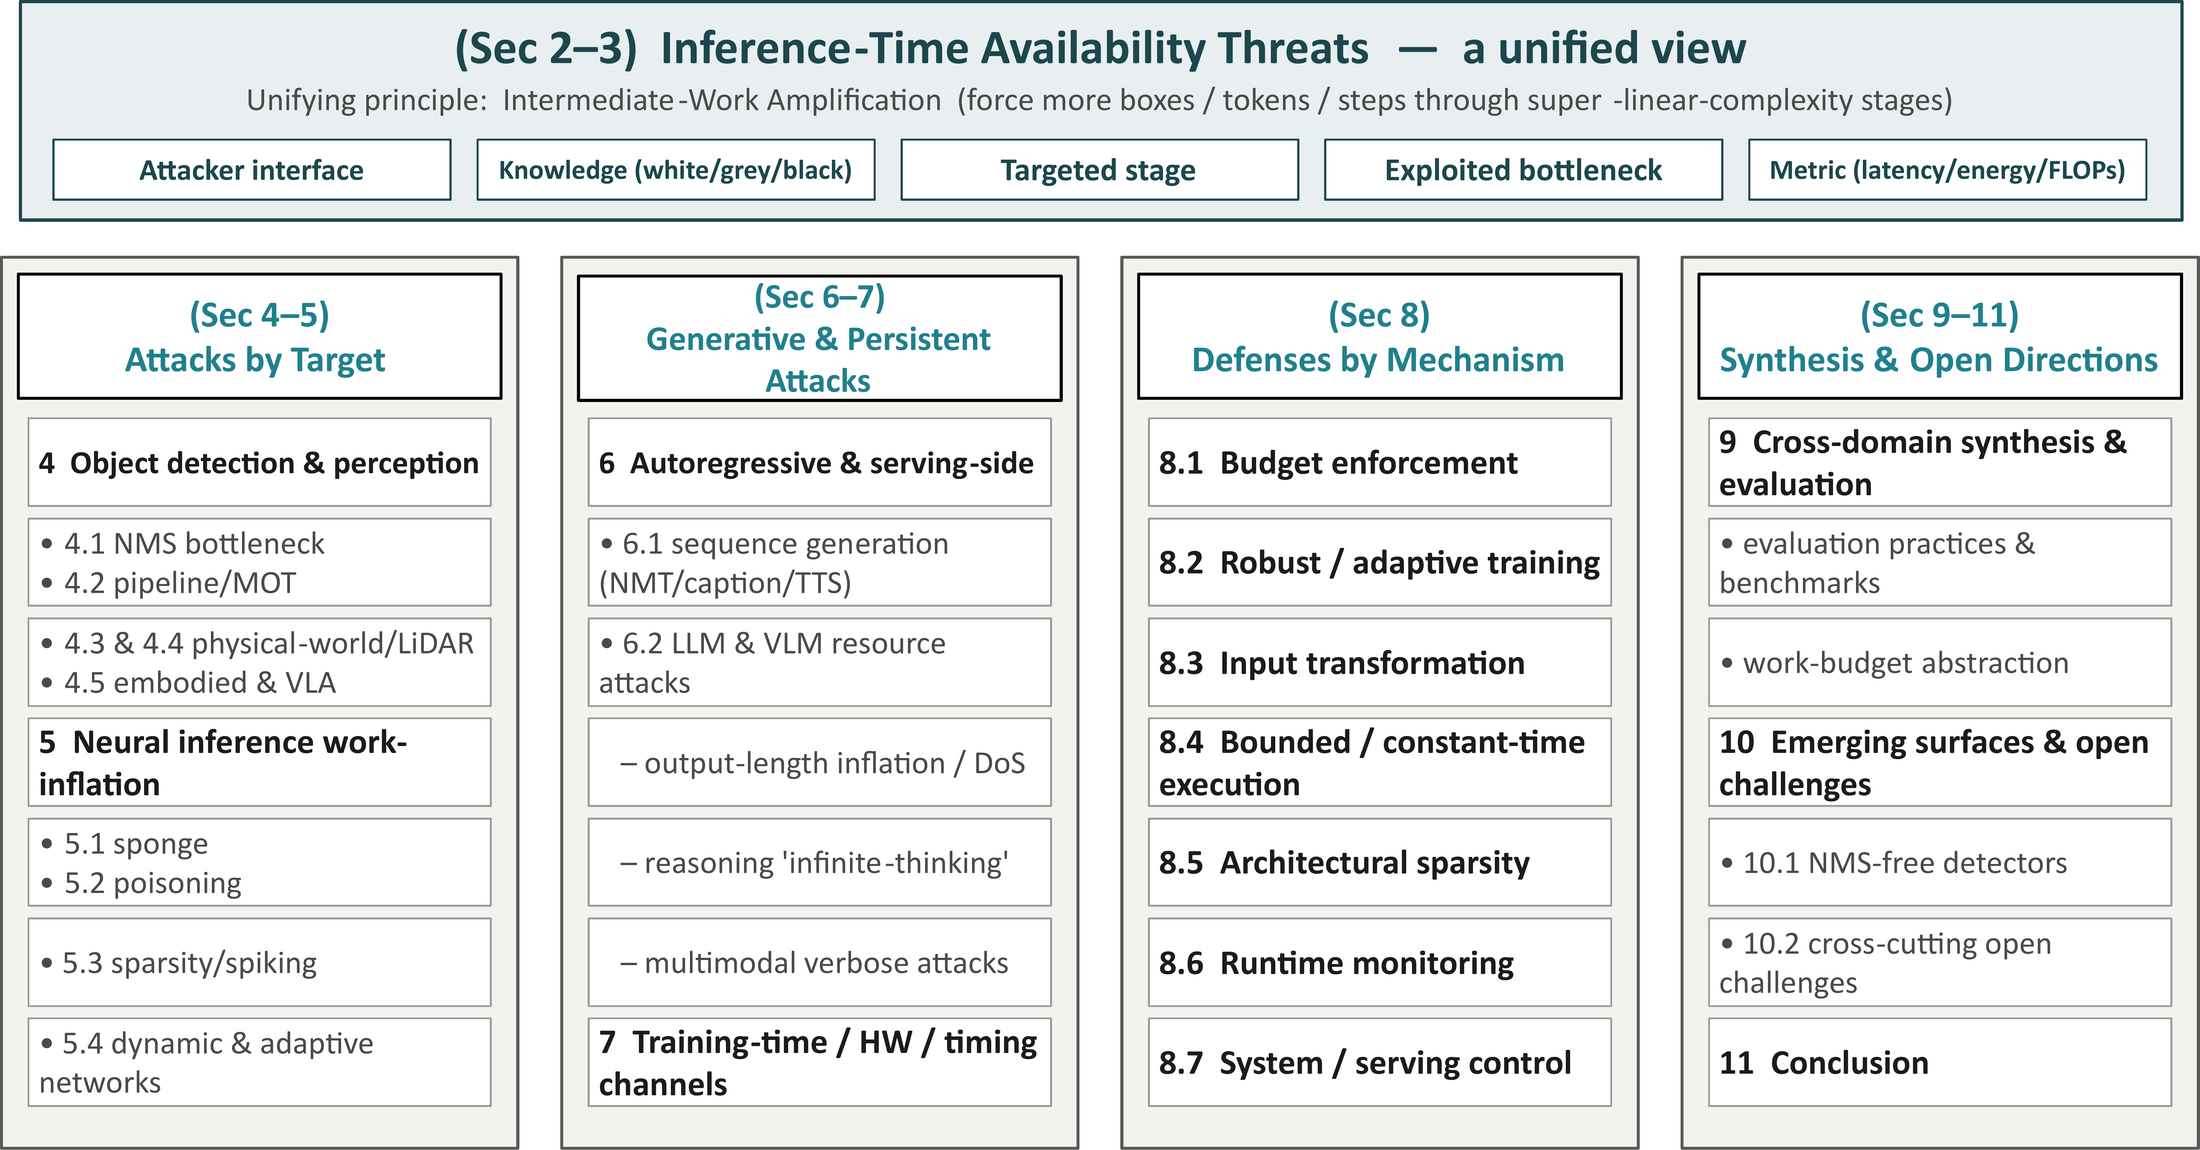
\includegraphics[width=\textwidth]{Figs/overview_structure.png}
  \caption{Overview of the survey structure.}
  \Description{A high-level structure diagram showing how the survey is organized.}
  \label{fig:survey-structure}
\end{figure*}

\subsection{Why latency attacks matter now}
Although many works surveyed in this paper are recent, the rapid expansion of latency attacks across perception, adaptive inference, and foundation models motivates a unified survey at this stage. Three trends have converged to make latency attacks a first-class concern. First, \emph{real-time autonomy} couples perception latency directly to physical safety: a delayed detection cascades into delayed planning and control~\cite{ma2024slowtrack}. Second, the field has embraced \emph{input-adaptive efficiency}---early-exit networks, token pruning, skimming transformers, and mixture-of-experts routing---which trade a fixed worst-case cost for a lower \emph{average} cost. This is precisely the property an availability attacker can revoke: by forcing every input onto the slow path, the attacker erases the advertised savings and may even exceed the cost of the static model~\cite{hong2021deepsloth,chen2023dynamic}. Third, the rise of \emph{autoregressive generation} in LLMs and VLMs means that a small input can induce an arbitrarily large output, and the per-query compute cost is now an attacker-controllable variable~\cite{gao2024verbose,dong2024engorgio}. The recent move to inference-time ``thinking'' in reasoning models multiplies this leverage: a single innocuous-looking prompt can trigger tens of thousands of reasoning tokens~\cite{liu2026reasoningbomb}.

\subsection{Scope and contributions}
Prior surveys treat pieces of this landscape in isolation. The closest, by Brachemi Meftah et al.~\cite{meftah2025survey}, covers energy-latency attacks on regular, input-adaptive, and decoder-based models, but predates and only shallowly covers the LLM/VLM era---reasoning-model denial-of-service, mixture-of-experts routing attacks, and multimodal verbose attacks. The autonomous-driving security literature, meanwhile, has produced a rich set of \emph{physically realizable} latency attacks that are rarely discussed alongside the general deep-learning work. This survey deliberately bridges both. We make the following contributions:



\begin{itemize}
  \item \textbf{A unified taxonomy} that organizes latency attacks by exploited bottleneck and by affected model class, spanning object detection, dynamic networks, transformers, LLMs, and multimodal generators.
  \item \textbf{A unifying principle}---\emph{intermediate-work amplification} (Section~\ref{sec:unifying})---that explains every attack class through a single mechanism and motivates a cross-domain \emph{work-budget} defense abstraction.
  \item \textbf{A threat-model framework} (Section~\ref{sec:threat}) that classifies the attacker interface, knowledge, and targeted pipeline stage, making otherwise incomparable works commensurable.
  \item \textbf{Consolidated quantitative comparisons} (Tables~\ref{tab:od-attacks}, \ref{tab:general-attacks}, \ref{tab:defenses}) of reported latency, energy, FLOP, and output-length amplification factors, with explicit notes on metric incompatibility.
  \item \textbf{A structured defense review} (Section~\ref{sec:defenses}) organized by control mechanism rather than by target, exposing which point of the compute pathway each defense actually bounds.
  \item \textbf{A cross-domain synthesis and evaluation discussion} (Section~\ref{sec:synthesis}) showing why perception-side and serving-side defenses do not transfer, including a review of fragmented evaluation practice (Section~\ref{sec:eval}).
  \item \textbf{A forward-looking analysis} (Section~\ref{sec:open}, including the NMS-free detector discussion in Section~\ref{sec:nmsfree}) of emerging attack surfaces and the open challenges that define the next phase of this research.
\end{itemize}

%% ===============Section 2==============================================
\section{Background and Definitions}
\label{sec:background}

\subsection{Integrity versus availability}

Deep learning is now pervasively deployed on resource-constrained embedded and edge platforms, where inference latency, energy, and throughput are first-class design constraints rather than afterthoughts~\cite{luo2024efficient,marco2020adaptive,kim2025emamba}. It is precisely in these latency- and energy-sensitive regimes that availability attacks become consequential. We adopt the NIST taxonomy of adversarial machine learning, which distinguishes integrity, availability, and confidentiality violations~\cite{vassilev2023nist}. Integrity attacks aim to change the model's output; availability attacks aim to degrade its usefulness or serviceability. Latency attacks are availability attacks whose specific lever is computational cost. Crucially, a latency attack may leave the prediction \emph{unchanged}---this is a feature, not a side effect, because output-quality monitors (BLEU for translation, mAP for detection, perplexity for text) will not flag an attack that only changes timing~\cite{chen2022nmtsloth,shapira2023phantom}. Gao et al. \cite{gao2026performance} evaluated and compared well-known certifiable defenses against adversarial patches across different hardware platforms with varying computing power in terms of both robust accuracy and processing time of the defense algorithm, which addresses availability attacks and is orthogonal to the availability attacks considered in this survey article.

%presented a comprehensive performance measurement and analysis of six certifiable defense algorithms
%against adversarial patch attacks, encompassing 14 models across three hardware platforms . Our results highlight a critical trade-off between robust accuracy and computational overhead, which is a primary consideration for deployment in real-time, resourceconstrained cyber-physical systems. In this study, we evaluate and compare six well-known certifiable adversarial patch defenses, encompassing 14 models, across three different hardware platforms. We analyze their performance in terms of accuracy and processing time, highlighting key trade-offs

\subsection{Where latency comes from}

A modern inference pipeline contains many cost centers, and latency attacks succeed by driving one or more toward its worst case:
\begin{description}
  \item[Data-dependent post-processing.] Operations whose cost depends on the \emph{content}, not just the shape, of intermediate tensors. The canonical example is non-maximum suppression (NMS) in object detectors, whose cost grows with the number of candidate boxes~\cite{shapira2023phantom}.
  \item[Activation sparsity.] Hardware accelerators (GPUs, TPUs, ASICs) exploit zero-valued activations to skip computation, and approximate-computing techniques trade accuracy for energy on the edge~\cite{ghosh2023approxedge}. Inputs that minimize sparsity force maximum multiply-accumulate work and energy~\cite{shumailov2021sponge,muller2024uniform}.
  \item[Conditional computation.] Early-exit networks, token-pruning vision transformers, skimming language models, and mixture-of-experts routers all decide \emph{at runtime} how much computation to perform~\cite{teerapittayanon2016branchynet,rao2021dynamicvit,fedus2022switch}; the same input-adaptive model-selection strategies that save average-case energy on embedded systems~\cite{marco2020adaptive} create the worst-case headroom an attacker can reclaim. Each decision point is an attack target.
  \item[Autoregressive generation.] Sequence models emit one token at a time until an end-of-sequence (EOS) signal. The number of tokens---and thus total cost---is determined by the model's own outputs, which the attacker can steer~\cite{chen2022nmtsloth,gao2024verbose}.
  \item[Temporal and multi-agent state.] Pipelines that maintain state across frames (multi-object tracking) or aggregate across agents (cooperative perception) add stages whose cost depends on the number of tracked or fused entities~\cite{jia2020fooling,wang2026cpfreezer}.
  \item[Hardware and memory.] Memory access patterns, DRAM bandwidth, and even induced bit-flips can be manipulated to inflate latency below the algorithmic level~\cite{sistla2025bitflip,nakai2021timing}.
\end{description}

\subsection{The unifying principle: intermediate-work amplification}
\label{sec:unifying}

Beneath the diversity of targets and modalities lies a single mechanism, which we call \emph{intermediate-work amplification}. In every latency attack, the adversary engineers a situation in which some internal boundary of the computation receives more objects, tokens, attention computations, or reasoning steps than a benign input of the same nominal class would generate. In object detection, those objects are phantom bounding boxes that flood NMS or multi-object tracking. In transformer inference, they are tokens that occupy the KV-cache and drive quadratic attention. In autoregressive decoding, they are extra generated tokens; in reasoning models, extra chain-of-thought steps. The attack is effective precisely because the relevant algorithms---NMS, self-attention, autoregressive decoding, Hungarian matching---have at least \emph{super-linear worst-case complexity} in the count of intermediate objects, so a modest increase in the count produces a disproportionate increase in cost. This shared structure appears across both perception pipelines and LLM/VLM-serving domains. This abstraction is more than descriptive: it implies that the natural cross-domain defense is a \emph{work budget}---an explicit cap on the number of intermediate objects, tokens, or attention computations permitted per unit time, enforced at the boundary between stages (Section~\ref{sec:synthesis}).

\begin{figure*}[htbp]
  \centering
  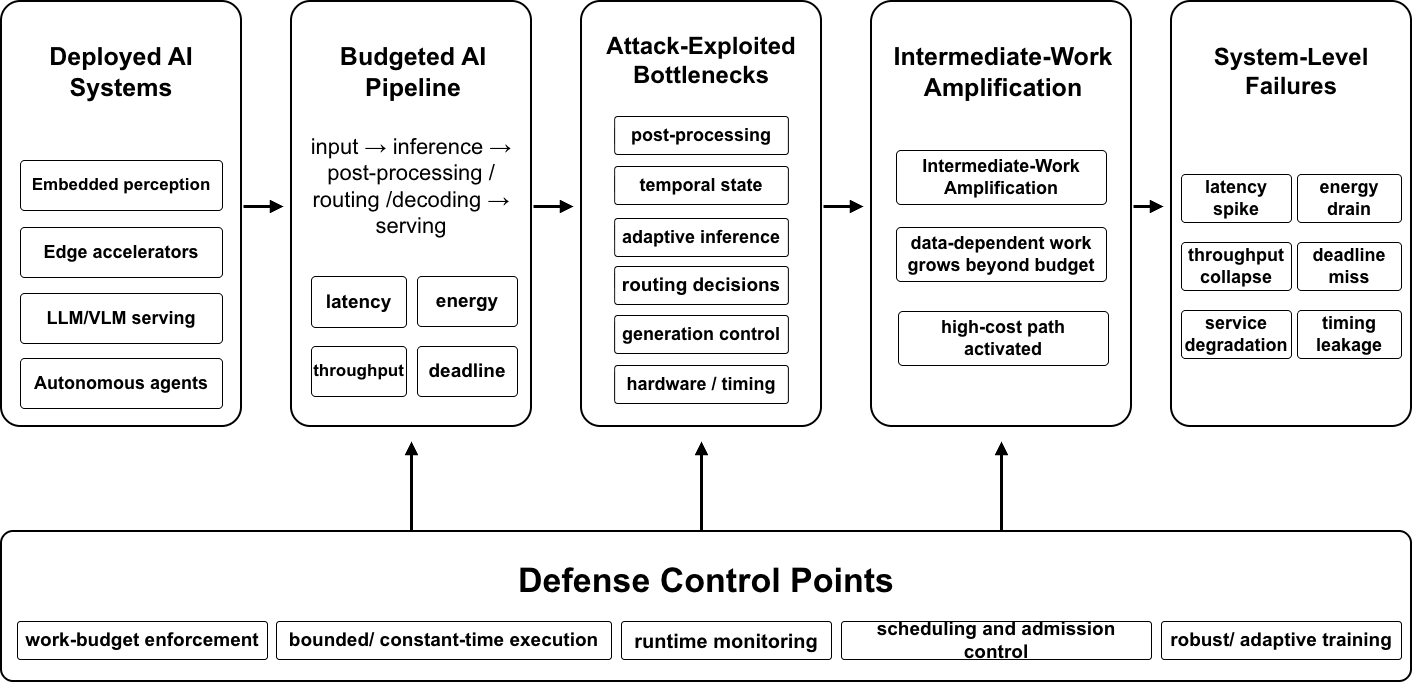
\includegraphics[width=\textwidth]{Figs/overview_system_availability_v4.png}
  \caption{Overview of latency attacks as system-level availability threats.}
  \Description{A system-level overview showing deployed AI systems, a budgeted AI pipeline, attack-exploited bottlenecks, intermediate-work amplification, system-level failures, and defense control points.}
  \label{fig:overview}
\end{figure*}

Figure~\ref{fig:overview} presents an overview of latency attacks as system-level availability threats. Deployed AI systems operate under latency, energy, throughput, and deadline budgets. Attackers exploit data-dependent bottlenecks to amplify intermediate work and push execution toward high-cost paths, causing latency spikes, energy drain, throughput collapse, missed deadlines, service degradation, or timing leakage. Defenses restore bounded and predictable computation through budget enforcement, monitoring, scheduling, and bounded execution. %We therefore focus below on the differences between attack families rather than repeating the taxonomy.

\subsection{Related surveys}
Adversarial-ML surveys overwhelmingly emphasize \emph{evasion}---perturbations that cause misclassification---and treat the availability axis as peripheral~\cite{liao2025llmsurvey,aguilera2025llmsecurity,chowdhury2024breakingdown}. Surveys of adversarial attacks on vision-language models catalog jailbreak, backdoor, and patch threats but largely omit output-length and resource-consumption attacks~\cite{hossain2026vlmsurvey,fu2025vlmdefense,dai2025vlmattacks}. LLM-security surveys catalog serving-layer availability attacks but do not connect them to the perception-stack latency literature~\cite{xu2025llmattacks}. Earlier work by Kianpour and Wen~\cite{kianpour2019timing} surveyed \emph{timing attacks} on ML systems and laid conceptual groundwork, but predates the NMS-overload and LLM-DoS literature. The closest dedicated treatment, Brachemi Meftah et al.~\cite{meftah2025survey}, covers energy-latency attacks on regular, adaptive, and decoder-based models but only addresses the LLM/VLM era in a shallow way. To our knowledge, this survey is the first to unify latency attacks and defenses across perception pipelines, dynamic networks, and LLM/VLM serving under a single threat model. Table~\ref{tab:surveys} positions our work against prior surveys along three coverage axes---autonomous-driving (AD) perception, general deep learning, and the LLM/VLM era---and identifies the principal gap each leaves open.

\begin{table}[htbp]
  \caption{Positioning of this survey against prior surveys touching latency, timing, or availability attacks. \CIRCLE: substantial coverage; \LEFTcircle: partial/peripheral coverage; \Circle: not covered.}
  \label{tab:surveys}
  \small
  \begin{tabularx}{\linewidth}{L{3.0cm} c c c c X}
    \toprule
    \textbf{Survey} & \textbf{Year} & \textbf{AD percep.} & \textbf{General DL} & \textbf{LLM/VLM} & \textbf{Principal gap} \\
    \midrule
    Kianpour \& Wen~\cite{kianpour2019timing} & 2019 & \Circle & \LEFTcircle & \Circle & Predates modern latency/sponge and LLM-DoS literature \\
    \addlinespace
    NIST AML taxonomy~\cite{vassilev2023nist} & 2023 & \Circle & \LEFTcircle & \LEFTcircle & Definitional only; availability is one small category \\
    \addlinespace
    LLM-security surveys~\cite{xu2025llmattacks,liao2025llmsurvey,aguilera2025llmsecurity,chowdhury2024breakingdown} & 2024--25 & \Circle & \Circle & \CIRCLE & Serving-layer DoS only; no link to perception latency \\
    \addlinespace
    VLM adversarial surveys~\cite{hossain2026vlmsurvey,fu2025vlmdefense,dai2025vlmattacks} & 2025--26 & \LEFTcircle & \Circle & \LEFTcircle & Jailbreak/backdoor/patch focus; omits output-length \& resource attacks \\
    \addlinespace
    Brachemi Meftah et al.~\cite{meftah2025survey} & 2025 & \LEFTcircle & \CIRCLE & \LEFTcircle & Shallow on LLM/VLM, reasoning, and MoE; no AD system-level synthesis \\
    \addlinespace
    \textbf{This survey} & 2026 & \CIRCLE & \CIRCLE & \CIRCLE & --- (unifies all three via intermediate-work amplification) \\
    \bottomrule
  \end{tabularx}
\end{table}

\subsection{A note on metrics}
Reported results in this field are often incomparable. Authors may report multiplicative latency increases ($\times$), absolute milliseconds, FLOP increases, energy in joules, generated-token counts, frames per second, and downstream task outcomes (crash rate, collision rate). On embedded targets, the relevant quantity is often the worst-case execution time relative to a real-time deadline, which has motivated dedicated execution-time prediction frameworks for concurrent DNN workloads on edge accelerators~\cite{goel2024express}. Throughout, we preserve each paper's native metric and flag where direct comparison is unsound. Establishing common axes is itself an open problem (Section~\ref{sec:open}).

%% ================Section 3=============================================
\section{Threat Models}
\label{sec:threat}
A coherent threat model is the prerequisite for comparing attacks that span sensor inputs, public APIs, and hardware faults; without it, headline slowdown numbers are not commensurable. We classify latency attacks along three dimensions: the \emph{attacker interface} (how the adversary touches the system), the \emph{attacker knowledge} (white-, grey-, or black-box), and the \emph{targeted stage}. Table~\ref{tab:threats} summarizes representative families.

\begin{table}[htbp]
  \caption{Threat-model families for latency attacks, with representative works.}
  \label{tab:threats}
  \small
  \begin{tabularx}{\linewidth}{L{2.4cm} L{2.6cm} L{3.0cm} X}
    \toprule
    \textbf{Family} & \textbf{Interface} & \textbf{Targeted stage} & \textbf{Representative evidence} \\
    \midrule
    Digital input perturbation & Modify sensor input (image, point cloud, text) & Detector inference / NMS / decoder & Overload~\cite{chen2024overload}; Phantom Sponges~\cite{shapira2023phantom}; sponge examples~\cite{shumailov2021sponge} \\
    \addlinespace
    Pipeline-level perturbation & Modify camera input for end-to-end effect & Full perception (detect + track) & SlowTrack~\cite{ma2024slowtrack} \\
    \addlinespace
    Physical projector / patch & Project or print patterns into the scene & Camera perception via phantom objects & SlowPerception~\cite{ma2024slowperception}; DetStorm~\cite{muller2025detstorm} \\
    \addlinespace
    Sensor runtime maximization & Perturb LiDAR point clouds & LiDAR detection runtime & SlowLiDAR~\cite{liu2023slowlidar} \\
    \addlinespace
    Cooperative V2V injection & Inject perturbations via V2V messages & Cooperative-perception fusion & CP-FREEZER~\cite{wang2026cpfreezer} \\
    \addlinespace
    Autoregressive inflation & Craft input prompt / image & Decoder generation length & NMTSloth~\cite{chen2022nmtsloth}; Engorgio~\cite{dong2024engorgio}; Verbose Images~\cite{gao2024verbose} \\
    \addlinespace
    Dynamic-control defeat & Craft input to defeat conditional compute & Early-exit / pruning / routing & DeepSloth~\cite{hong2021deepsloth}; No-Skim~\cite{zhang2023noskim}; Misrouter~\cite{fei2026misrouter} \\
    \addlinespace
    Training-time poisoning & Poison training data or weights & Persistent inference cost & Sponge poisoning~\cite{cina2022sponge}; SkipSponge~\cite{telintelo2024skipsponge}; DoS poisoning~\cite{gao2024dospoisoning} \\
    \addlinespace
    Hardware / side-channel & Induce faults or observe timing & NMS / memory / timing oracle & Bit-flip attack~\cite{sistla2025bitflip}; timing side-channel~\cite{nakai2021timing} \\
    \bottomrule
  \end{tabularx}
\end{table}

\subsection{Attacker interface}
The interface ranges from purely digital (modifying the input tensor of a model under white-box control) to physical (projecting or printing adversarial patterns that a camera then captures) to systemic (injecting messages over a vehicle-to-vehicle channel, or submitting prompts to a public API). Physical realizability is the dividing line between laboratory demonstrations and deployable threats, and is a recurring theme in the autonomous-driving literature~\cite{ma2024slowperception,muller2025detstorm}.

\subsection{Attacker knowledge}
White-box attacks assume gradient access and dominate early work because the optimization is direct. Grey-box attacks assume architectural knowledge but not exact weights~\cite{du2024energy}. Black-box attacks, increasingly important for deployed services, rely on transfer from a surrogate, on query feedback (e.g., \texttt{usage.prompt\_tokens}), or even on timing itself as an oracle~\cite{nakai2021timing,zhang2025crabs}. The existence of timing-only black-box attacks is significant: it means even an opaque service that returns no probabilities can leak enough information to be optimized against.

%% =================Section 4============================================
\section{Latency Attacks on Object Detection and Perception}
\label{sec:od}
Object detection is the most thoroughly studied target, because its post-processing stage offers an unusually clean computational bottleneck and because autonomous driving supplies a high-stakes deployment context.

\subsection{Non-maximum suppression as a bottleneck}
NMS filters overlapping candidate boxes and has a cost that grows with the number of candidates. \emph{Phantom Sponges}~\cite{shapira2023phantom} crafts a universal adversarial perturbation that adds many ``phantom'' boxes to overload NMS while \emph{preserving} the original detections, so accuracy collapse does not betray the attack. \emph{Overload}~\cite{chen2024overload} generalizes this by formulating latency maximization as an optimization with a spatial-attention mechanism, reporting that single-image inference time can be increased tenfold, and emphasizing that the attack is ``NMS-agnostic.'' \emph{Beyond PhantomSponges}~\cite{schoof2024beyond} modifies a box-area loss to lower intersection-over-union and exacerbate NMS load, reporting up to a 550\% increase in NMS time on a YOLOv5-small configuration. \emph{Groundswell}~\cite{xia2026groundswell} sharpens the stealth--effectiveness tradeoff with a \emph{Regional Perturbation Balance} strategy that injects phantom objects into spatial regions that minimally disturb the original detections; on YOLOv5s it inflates the candidate count fed to NMS from 101 to roughly 19{,}000 and end-to-end latency from 15.2~ms to 41.4~ms (about a 172\% increase), while cutting optimization time by 80\% relative to prior universal-perturbation attacks. \emph{Daedalus}~\cite{wang2019daedalus}, although framed as an integrity attack, is a relevant NMS failure mode: it compresses box dimensions so NMS cannot filter dense false positives, and is demonstrated via printed posters. A complementary observation by Biton et al.~\cite{biton2023timing} reframes variable-time inference as a security liability in itself: because NMS runtime is data-dependent, it \emph{leaks} internal inference state, and this timing signal can be used to enhance black-box, decision-based attacks. This dual role---NMS as both a target of latency inflation and a side-channel oracle---motivates constant-time NMS as an explicit security requirement (Section~\ref{sec:defenses}).
%(e.g., raising SORT latency to 1{,}082~ms versus 411~ms for Overload) 

\subsection{Whole-pipeline and temporal-state attacks}
Detector-only attacks often fail to change downstream behavior because multi-object tracking (MOT) absorbs detection noise; prior work shows that over 98\% detection-attack success may be required to alter tracking outcomes~\cite{jia2020fooling}. This motivates pipeline-level threat models. \emph{SlowTrack}~\cite{ma2024slowtrack} attacks camera-based perception end to end with a two-stage strategy and three new loss designs, reporting average latency $2.9\times$ higher than prior approaches for latency of the whole camera-based AD perception system; and, critically, connecting latency to safety: a vehicle crash rate of $\sim$95\% versus $\sim$30\% for baselines, evaluated on the Baidu Apollo stack and LGSVL simulator. Related temporal-integrity work---tracker hijacking~\cite{jia2020fooling,ma2023wip} and trajectory-aware attacks on MOT~\cite{hu2026trajectory}---reinforces that stateful components can amplify or attenuate component-level perturbations.

\subsection{Physical-world latency attacks}
\emph{SlowPerception}~\cite{ma2024slowperception} introduces projector-based universal perturbations that create numerous phantom objects, inducing an average physical-world latency of 2.5~seconds and a 97\% collision rate in an industry-grade system plus simulator. \emph{DetStorm}~\cite{muller2025detstorm} advances physical realizability, optimizing objects against multiple NMS variants and reporting a 506\% average increase in detected objects and delays up to 8.1~seconds, while arguing that prior digital or large-patch attacks lack real-world applicability. \emph{Groundswell}~\cite{xia2026groundswell} is explicitly designed for physical delivery: the universal perturbation can be affixed as a sticker on the camera lens or projected onto a surface ahead of the vehicle, injecting itself into raw frames before in-vehicle processing and pushing per-frame latency past the 30~ms real-time budget required by Level-4/5 autonomy.

\subsection{Beyond cameras: LiDAR and cooperative perception}
\emph{SlowLiDAR}~\cite{liu2023slowlidar} presents the first systematic availability attack on LiDAR detection, handling non-differentiable preprocessing via differentiable proxies and an execution-time-aware loss to inflate runtime across six popular pipelines while maintaining imperceptibility. \emph{CP-FREEZER}~\cite{wang2026cpfreezer} targets vehicular cooperative perception, injecting adversarial perturbations via V2V messages to maximize fusion delay; it resolves point-cloud nondifferentiability and transmission asynchrony, increasing end-to-end latency by over $90\times$, pushing per-frame time beyond 3~seconds, and achieving 100\% success on a real vehicle testbed. A simulation study further analyzes the system-level impact of perception inference-time attacks on full autonomous vehicle stacks~\cite{chen2025impact}, and real-time defenses against object-based LiDAR attacks are beginning to appear~\cite{zhang2025detstormlidar}.

\begin{table}[htbp]
  \caption{Representative latency attacks on object detection and perception. Metrics are reported as in the source; ``--'' indicates not reported in a directly comparable form.}
  \label{tab:od-attacks}
  \small
  \begin{tabularx}{\linewidth}{L{2.5cm} L{2.6cm} X L{2.0cm}}
    \toprule
    \textbf{Method} & \textbf{Target stage} & \textbf{Key quantitative result} & \textbf{Physical?} \\
    \midrule
    Phantom Sponges~\cite{shapira2023phantom} & NMS (end-to-end OD) & Universal perturbation overloads NMS while preserving detections & No \\
    Overload~\cite{chen2024overload} & OD inference (edge) & Single-image inference time up to $10\times$; NMS-agnostic & Edge-eval \\
    Beyond PhantomSponges~\cite{schoof2024beyond} & NMS runtime (YOLO) & Up to 550\% NMS-time increase (YOLOv5-small) & No \\
    Groundswell~\cite{xia2026groundswell} & NMS (camera OD) & Candidates 101$\to$19k; 15.2$\to$41.4~ms ($\sim$172\%); $-$80\% opt.\ time & Yes (sticker/projector) \\
    SlowTrack~\cite{ma2024slowtrack} & Camera perception (detect+track) & Latency $2.9\times$ vs.\ prior; crash rate $\sim$95\% vs.\ $\sim$30\% & Patch (prelim.) \\
    SlowPerception~\cite{ma2024slowperception} & NMS + MOT workload & Avg.\ 2.5~s physical latency; 97\% collision rate & Yes (projector) \\
    DetStorm~\cite{muller2025detstorm} & Camera perception delay & 506\% more detections; up to 8.1~s delay & Yes \\
    SlowLiDAR~\cite{liu2023slowlidar} & LiDAR detection runtime & Significant latency rise on six LiDAR pipelines & No \\
    CP-FREEZER~\cite{wang2026cpfreezer} & Cooperative fusion & $>90\times$ latency; $>$3~s/frame; 100\% on testbed & Yes (testbed) \\
    Sponge Backdoor~\cite{xiao2024sponge} & OD latency via NMS & Poisoned inputs prolong time; clean accuracy preserved & No \\
    Bit-flip attack~\cite{sistla2025bitflip} & NMS via parameters & Up to 71.6~ms ($20.4\times$) with 31 bit-flips & Partial \\
    \bottomrule
  \end{tabularx}
\end{table}

\subsection{Embodied and Vision-Language-Action Availability Attacks}
\label{sec:vla}
The latest frontier moves past the perception front-end to the \emph{Vision-Language-Action} (VLA) models that map multimodal observations directly to robot actions, where an availability failure is a physical failure: a robot that stalls or acts late can collide, drop a payload, or freeze mid-manipulation. \emph{FreezeVLA}~\cite{wang2025freezevla} formalizes \emph{action-freezing} attacks via min-max bi-level optimization: a single adversarial image ``freezes'' the VLA and makes it ignore subsequent instructions---disconnecting the robot's digital mind from its physical actions---attaining a $76.2\%$ average freeze rate across three VLA models and four benchmarks, with strong cross-prompt transferability. \emph{Semantic-DoS}~\cite{steinberg2026semanticdos} turns the model's own safety alignment into the attack surface: injecting short (1--5 token) safety-plausible phrases into the robot's audio channel triggers protective halting without any jailbreak, reaching up to $98.3\%$ hard-stop success and revealing that prompt-level defenses merely reshape---rather than remove---the disruption. Patch-based variants such as the Embedding Disruption Patch Attack (\emph{EDPA})~\cite{xu2025edpa} place a model-agnostic patch in the camera view that breaks visual--textual alignment and drives repeated incorrect actions to task failure, and \emph{MAVLA}~\cite{zhao2026mavla} breaks cross-modal alignment through a coordinated multimodal adversarial framework. \emph{ANNIE}~\cite{huang2025annie} provides the first systematic, ISO-grounded study of embodied safety violations, decomposing long-horizon goals into frame-level perturbations and exceeding $50\%$ success across critical, dangerous, and risky categories with validation on a physical robot. These attacks share the availability signature of the rest of this survey---worst-case work or worst-case delay imposed on a real-time loop---but relocate the consequence from a slow inference to an unsafe or absent physical action; broader treatments of the embodied threat surface are emerging in dedicated surveys~\cite{xing2025embodiedsurvey}.

\textbf{Section Summary.} Collectively, these studies illustrate a clear evolution of latency attacks in perception systems. Early work primarily exploited a single computational bottleneck, most notably non-maximum suppression (NMS). More recent research increasingly targets complete perception pipelines, incorporates physical realizability, and evaluates downstream consequences such as tracking failures, delayed planning, and collision risk---and, most recently, extends to the embodied VLA policies that consume perception output, where induced latency or action-freezing becomes a direct physical hazard. This progression suggests that latency attacks are evolving from component-level vulnerabilities into system-level threats that must be evaluated across the entire autonomy stack. More importantly, the object-detection literature also reveals a broader lesson: although NMS happened to be the first successful target, the underlying objective is not to attack NMS itself, but to maximize intermediate computation wherever it occurs. The following sections show that the same principle extends naturally to activation sparsity, adaptive inference, autoregressive generation, and LLM serving.

%Section Summary. Collectively, these studies illustrate a clear evolution of latency attacks in perception systems. Early work primarily exploited a single computational bottleneck, most notably non-maximum suppression (NMS). More recent research increasingly targets complete perception pipelines, incorporates physical realizability, and evaluates downstream consequences such as tracking failures, delayed planning, and collision risk. More importantly, this evolution suggests that the attacker’s objective is not to exploit NMS specifically, but to maximize intermediate computation wherever it occurs. This observation naturally motivates the broader work-inflation perspective developed in the following sections.

%% ===================================================================
\section{Neural Inference Work-Inflation Attacks}
\label{sec:sponge}

The \emph{sponge} lineage targets the general mechanism of activation sparsity rather than any specific post-processing stage, making it broadly applicable across architectures.

\subsection{Inference-time sponge examples}
\emph{Sponge examples}~\cite{shumailov2021sponge} are the seminal work: adversarial inputs crafted to maximize energy and latency by minimizing the activation sparsity that accelerators exploit. On transformer and vision models, they report up to $30\times$ increases in latency and energy consumption in some settings, and a real-world demonstration that raised a cloud translator's response time from 1~ms to 6~s. A follow-up analysis shows that uniform/constant inputs act as ``free'' sponge examples and that the achievable energy increase is bounded by the architecture's sparsity range, motivating activation-sparsity monitoring as a defense signal~\cite{muller2024uniform}.

\subsection{Sponge poisoning: moving the attack to training}
\emph{Sponge poisoning}~\cite{cina2022sponge} injects a small fraction of crafted samples so the trained model incurs elevated energy on \emph{all} natural inputs thereafter---a far stealthier and more persistent variant. \emph{SkipSponge}~\cite{telintelo2024skipsponge} operates directly on weights, poisoning residual (skip) connections with under 1\% weight modification and evading fine-pruning and parameter-perturbation defenses. Sponge poisoning has been adapted to on-device DNNs~\cite{wang2023ondevice}, to multi-exit networks (where it both prevents early exits and raises per-layer cost)~\cite{huang2024multiexit}, to mobile apps~\cite{paul2023mobile}, and to FPGA accelerators under differential privacy~\cite{akram2025evoweight}. A sensing-AI study quantifies battery-drain risk in IoT settings and proposes pruning as a defense, reducing energy overhead from $\sim$4$\times$ to $\sim$1.3$\times$~\cite{hasan2025sensing}.

\subsection{Sparsity and spiking networks}
\emph{Sparsity attacks}~\cite{krithivasan2020sparsity} degrade energy/latency by minimizing activation sparsity and withstand activation thresholding and input quantization. Spiking neural networks, attractive for low-power edge perception, are also vulnerable: efficiency attacks raise spike activity by $1.7\times$--$2.5\times$ and energy by $1.4\times$--$2.2\times$~\cite{krithivasan2022spikeattack}, and timestep-compressed methods reduce the latency of \emph{generating} such attacks for real-time use~\cite{kang2025tca}.

%% ===================================================================
\subsection{Dynamic and Adaptive Networks}
\label{sec:dynamic}

Input-adaptive networks promise lower \emph{average} cost; latency attacks revoke that promise by forcing worst-case control flow.

\noindent\textbf{Multi-exit networks.}
The earliest availability attack on input-adaptive networks is \emph{ILFO}~\cite{haque2020ilfo}, which optimizes an intermediate-output loss to reactivate skipped blocks in depth-adaptive networks, increasing FLOPs by up to $100\%$. \emph{DeepSloth}~\cite{hong2021deepsloth} is the foundational slowdown attack on early-exit inference: per-input perturbations force the network to defer to its final, most expensive classifier, eliminating the efficiency advantage with 90--100\% success and up to $5.2\times$ cost inflation. Refined energy attacks combine energy maximization with confidence minimization and remain effective in grey-box settings~\cite{du2024energy}. In NLP, \emph{SlowBERT}~\cite{zhang2023slowbert} attacks multi-exit BERT, and \emph{Dynamic Transformers Provide a False Sense of Efficiency}~\cite{chen2023dynamic} introduces a unified attack (SAME) that defeats early exits across BERT, RoBERTa, ALBERT, and DistilBERT with up to $5\times$ slowdown. A foundational study demystifies \emph{why} these models are vulnerable and proposes calibration-based defenses that recover roughly 60\% of lost efficiency~\cite{varma2024slowdown}.

%Mixture-of-experts routers, central to modern sparse LLMs, are a fresh target: \emph{RouteHijack}~\cite{xu2026routehijack} concentrates tokens on expensive experts, and \emph{Misrouter}~\cite{fei2026misrouter} causes routing collapse or saturation in a black-box, query-only setting, both yielding $2$--$4\times$ latency increases. 

\noindent\textbf{Token pruning, skimming, and mixture-of-experts.}
Skimming language models drop unimportant tokens; \emph{No-Skim}~\cite{zhang2023noskim} crafts inputs that prevent dropping, raising FLOPs by $2$--$3\times$. A unified framework treats early exit, token-pruning vision transformers, and MoE routing as instances of one ``efficiency attack'' class, demonstrating $2$--$8\times$ overhead across all three~\cite{rathnasuriya2025ddls}. In the vision-transformer setting specifically, \emph{SlowFormer}~\cite{navaneet2024slowformer} trains a universal adversarial patch (as little as $2\%$ of the image area) that drives efficient ViTs such as A-ViT, ATS, and AdaViT toward their maximum compute, and \emph{QuantAttack}~\cite{baras2025quantattack} exploits dynamic quantization to force worst-case high-precision execution, inflating inference time, memory, and energy. Mixture-of-experts routers, central to modern sparse LLMs, are a fresh target: \emph{Misrouter}~\cite{fei2026misrouter} causes routing collapse or saturation in a black-box, query-only setting, yielding $2$--$4\times$ latency increases, while \emph{RouteHijack}~\cite{xu2026routehijack}---though primarily a jailbreak attack---demonstrates that adversarial control of expert routing can additionally inflate computation by activating costly experts. \emph{RepetitionCurse}~\cite{huang2025repetitioncurse} shows the vulnerability is systemic rather than incidental: under expert parallelism, simple repetitive-token prompts force all tokens onto the same top-$k$ experts, creating device-level bottlenecks while others idle and raising end-to-end latency by $3.06\times$ on Mixtral-8x7B---turning the efficiency mechanism itself into a denial-of-service vector. \emph{SPLAT}~\cite{li2026splat} revisits latency attacks on dynamic networks with a black-box, stealthy formulation for multi-exit models.

\textbf{Section Summary.} Unlike perception attacks, sponge attacks reveal that latency vulnerabilities are not tied to a particular application or post-processing stage. Instead, they exploit architectural properties shared by many neural networks, including activation sparsity and conditional computation. Training-time variants further demonstrate that excessive computational cost can be embedded persistently into model parameters rather than triggered solely by adversarial inputs. Taken together, these studies shift the focus from application-specific bottlenecks toward general properties of efficient neural inference.
%% ============Section 6================================================
\section{Autoregressive and Serving-Side Work Inflation}
\label{sec:seqgen}

\subsection{Sequence Generation and Decoder-Length Inflation}

Autoregressive decoders introduce a uniquely powerful lever: the attacker can inflate the \emph{number of generated tokens}, and total cost scales with it.

\emph{NMTSloth}~\cite{chen2022nmtsloth} is the first systematic study of efficiency robustness in neural machine translation, crafting source sentences that inflate decoder steps by $5$--$10\times$ and end-to-end latency by $3$--$8\times$ while leaving BLEU nearly unchanged so no quality monitor fires. \emph{LLMEffiChecker}~\cite{feng2022llmeffichecker} extends this to general LLMs, finding them \emph{more} vulnerable: a five-token perturbation can inflate generation length by $10$--$30\times$. \emph{NICGSlowDown}~\cite{chen2022nicgslowdown} brings the paradigm to neural image captioning, forcing decoders to emit far longer captions via image perturbations, and establishes a widely reused efficiency-robustness benchmark. \emph{TTSlow}~\cite{gao2024ttslow} demonstrates that the threat reaches audio: adversarial text inflates autoregressive text-to-speech decoding by up to $5\times$. The common thread---and a recurring defensive blind spot---is that none of these attacks degrade output quality, so they evade quality-based detection entirely.

%% ===================================================================
\subsection{LLM and VLM Resource-Consumption Attacks}
\label{sec:llm}


The LLM/VLM era both inherits the autoregressive lever and adds new ones: chain-of-thought reasoning, multimodal inputs, and shared serving infrastructure. The emergence of reasoning models fundamentally changes the threat landscape. Earlier latency attacks manipulated inference pipelines whose computational cost was largely bounded. Modern reasoning models intentionally expose computation as an input-dependent resource, giving attackers much greater leverage.

\noindent\textbf{Output-length inflation and inference-cost DoS.}
\emph{Engorgio}~\cite{dong2024engorgio} optimizes prompts that coerce LLMs into babbling, inflating output token counts by $10$--$50\times$ and transferring to black-box targets. \emph{Crabs}~\cite{zhang2025crabs} automates black-box LLM-DoS prompt generation, sustaining $10$--$30\times$ output inflation even under provider-side length monitoring through semantic camouflage. \emph{Denial-of-Service Poisoning}~\cite{gao2024dospoisoning} shows the threat can be embedded at training time: a triggered model emits endless output, never producing EOS, with 100\% success at under 1\% poisoning and survival through RLHF safety tuning.

\noindent\textbf{Reasoning-model and ``infinite-thinking'' attacks.}
Inference-time compute scaling creates a new, high-leverage surface. \emph{ReasoningBomb}~\cite{liu2026reasoningbomb} induces pathologically long reasoning traces in large reasoning models---averaging $\sim$18{,}759 completion tokens versus $\sim$300 for normal queries, a roughly $60\times$ cost multiplier---while remaining stealthy and bypassing input-, output-, and joint-detection baselines at rates of 99.8\%, 98.7\%, and 98.4\%, respectively. \emph{ThinkTrap}~\cite{li2026thinktrap} exploits chain-of-thought mode in black-box APIs to induce near-infinite thinking loops, consuming $50$--$100\times$ more tokens than standard requests. These results strongly argue  for budget enforcement through \emph{construction} rather than detection.

\noindent\textbf{Multimodal verbose attacks.}
\emph{Verbose Images}~\cite{gao2024verbose} crafts adversarial images that make large VLMs (GPT-4V, LLaVA, InstructBLIP, MiniGPT-4) generate long, repetitive responses, inflating output by $10$--$30\times$ and latency by $7$--$30\times$ while preserving visual fidelity. \emph{VLMInferSlow}~\cite{wang2025vlminferslow} provides a service-oriented evaluation across 12 open and closed VLMs, reporting 85--100\% success and $5$--$40\times$ increases in latency. \emph{Verbose-Text Induction}~\cite{luo2025verbosetext} co-optimizes adversarial images and prompts to exceed 10{,}000 output tokens from a single query, and \emph{LingoLoop}~\cite{fu2025lingoloop} traps multimodal models in self-referential generation loops that fill the context window faster than legitimate output, defeating context-length caps. The trajectory from image captioning~\cite{chen2022nicgslowdown} through verbose images to multimodal loop attacks is a coherent and accelerating escalation. This escalation now extends to the temporal domain: \emph{VidDoS}~\cite{tang2026viddos} is the first universal energy-latency attack tailored for video-based LLMs, using a single instance-agnostic adversarial patch---trained via masked teacher forcing with a refusal penalty and early-termination suppression---that requires no inference-time gradients and therefore keeps pace with continuous video streams. It induces token expansion exceeding $205\times$ and latency inflation exceeding $15\times$ across three Video-LLMs, and simulations of real-time autonomous-driving streams show the induced latency causes critical safety violations. The threat has also reached \emph{embodied} multimodal autonomy: a natural-reflection backdoor attack on driving VLMs~\cite{liu2025vlmbackdoor} embeds reflection-pattern triggers in camera images that, when present, cause the VLM planner to generate abnormally long responses---demonstrating significantly increased inference latency under trigger with direct real-world safety implications, and uniting the output-length-inflation and training-time-backdoor threat classes in a single AD-relevant attack.

\noindent\textbf{Serving-framework, tool-chain, and agentic DoS.}
The newest attacks move below the model to the \emph{serving system} and the \emph{agentic loop}, where shared infrastructure amplifies a single adversary's leverage. \emph{Fill and Squeeze}~\cite{wang2026fillsqueeze} reports the counter-intuitive finding that continuous batching largely neutralizes purely algorithmic length attacks, then attacks the scheduler directly---exhausting the global KV cache to induce head-of-line blocking and forcing repetitive preemption---for up to $20$--$280\times$ time-to-first-token slowdown in a black-box setting at lower cost than input-only methods. At the agent layer, \emph{Beyond Max Tokens}~\cite{zhou2026beyondmaxtokens} exploits the Model Context Protocol tool interface: text-only edits to tool metadata, optimized by Monte-Carlo tree search, steer agents into prolonged tool-calling chains exceeding 60{,}000 tokens, raising per-query cost by up to $658\times$ while preserving task success and evading prompt filters. \emph{From Shield to Target}~\cite{zhou2026shieldtarget} turns LLM \emph{guardrails} into the victim: crafted payloads trap the guardrail in extended reasoning loops for $13$--$63\times$ token amplification and up to $148\times$ latency amplification, and a single poisoned document can starve co-located agents sharing the guardrail. \emph{Mobius Injection}~\cite{liang2026mobius} generalizes this to agent-based DDoS (AbO-DDoS): by exploiting a ``semantic closure'' vulnerability, one textual injection induces sustained recursive agent execution, driving single-node call amplification up to $51\times$ and multi-node p95 latency up to $229\times$. These developments echo the broader systematization of the agentic attack surface~\cite{dehghantanha2026sokagentic} and are now recognized at the standards level as ``unbounded consumption''~\cite{owasp2025unbounded}---confirming that availability, not just integrity, is a first-class security property of deployed LLM services.

\begin{table}[htbp]
  \caption{Representative latency/energy attacks beyond object detection. Native metrics preserved.}
  \label{tab:general-attacks}
  \small
  \begin{tabularx}{\linewidth}{L{2.4cm} L{2.4cm} X}
    \toprule
    \textbf{Method} & \textbf{Domain / target} & \textbf{Key quantitative result} \\
    \midrule
    Sponge Examples~\cite{shumailov2021sponge} & General DNN (vision, NLP) & Up to $30\times$ energy/latency; cloud translator 1~ms$\to$6~s \\
    Sponge Poisoning~\cite{cina2022sponge} & Training-time, general & 1--5\% poison $\Rightarrow$ persistent $2$--$10\times$ energy \\
    SkipSponge~\cite{telintelo2024skipsponge} & Weight poisoning & High energy overhead at $<$1\% weight change; evades defenses \\
    DeepSloth~\cite{hong2021deepsloth} & Multi-exit networks & 90--100\% force full inference; up to $5.2\times$ cost \\
    Dynamic Transformers (SAME)~\cite{chen2023dynamic} & Multi-exit NLP & Up to $5\times$ slowdown across BERT family \\
    No-Skim~\cite{zhang2023noskim} & Skimming LMs & $2$--$3\times$ FLOPs; output label unchanged \\
    Misrouter~\cite{fei2026misrouter} & MoE routing (black-box) & $2$--$4\times$ latency via routing collapse/saturation \\
    RepetitionCurse~\cite{huang2025repetitioncurse} & MoE expert parallelism & $3.06\times$ latency on Mixtral-8x7B via router imbalance \\
    NMTSloth~\cite{chen2022nmtsloth} & Neural machine translation & $5$--$10\times$ decoder steps; $3$--$8\times$ latency; BLEU stable \\
    NICGSlowDown~\cite{chen2022nicgslowdown} & Image captioning & $5$--$10\times$ decoding steps; $3$--$7\times$ latency \\
    Engorgio~\cite{dong2024engorgio} & LLM prompts & $10$--$50\times$ output tokens; black-box transfer \\
    Crabs~\cite{zhang2025crabs} & LLM-DoS (black-box) & $10$--$30\times$ output; evades length monitoring \\
    ReasoningBomb~\cite{liu2026reasoningbomb} & Reasoning models & $\sim$60$\times$ tokens; $>$98\% detection bypass \\
    Verbose Images~\cite{gao2024verbose} & VLMs & $10$--$30\times$ output; $7$--$30\times$ latency \\
    VLMInferSlow~\cite{wang2025vlminferslow} & VLM-as-a-service & 85--100\% success; $5$--$40\times$ latency \\
    Fill and Squeeze~\cite{wang2026fillsqueeze} & LLM serving scheduler & $20$--$280\times$ TTFT slowdown; black-box \\
    Beyond Max Tokens~\cite{zhou2026beyondmaxtokens} & LLM agent tool chains (MCP) & Up to $658\times$ per-query cost; $>$60k-token chains \\
    From Shield to Target~\cite{zhou2026shieldtarget} & LLM guardrails & $13$--$63\times$ tokens; up to $148\times$ latency \\
    Mobius Injection~\cite{liang2026mobius} & Agentic AbO-DDoS & $51\times$ call amplification; $229\times$ p95 latency \\
    \bottomrule
  \end{tabularx}
\end{table}
%The emergence of autoregressive generation fundamentally changes the nature of latency attacks.
\textbf{Section Summary.}  Earlier attacks were constrained by the computational graph of a fixed model, whereas modern sequence models expose output length—and increasingly reasoning length—as attacker-controllable variables. As a result, computation itself becomes part of the attack surface. This transition explains why resource-consumption attacks have rapidly expanded from machine translation and image captioning to LLMs, VLMs, reasoning models, and mixture-of-experts architectures.

%% ==============Section 7===============================================
\section{Training-Time Persistence, Hardware, and Timing Channels}
\label{sec:hw}
%The attacks discussed in this section broaden the threat model beyond adversarial inputs. Computational overhead can be introduced during training, manipulated below the algorithmic level through hardware faults, or even exploited as an information leak through timing channels.
Not all latency attacks act on the test-time input. The attacks discussed in this section broaden the threat model beyond the test-time input: they persist across sessions, operate below the algorithm, or turn latency itself into an information leak, and are therefore the hardest to detect and remove. \emph{Training-time} variants (sponge poisoning~\cite{cina2022sponge}, SkipSponge~\cite{telintelo2024skipsponge}, sponge backdoors in detectors~\cite{xiao2024sponge}, and no-EOS DoS poisoning of LLMs~\cite{gao2024dospoisoning}) introduce persistent cost inflation that persists through normal usage and is hard to remove without retraining. \emph{Hardware} attacks operate below the algorithm: a row-hammer bit-flip approach targets NMS parameters via side channels, reporting up to 71.6~ms ($20.4\times$) latency with just 31 bit-flips~\cite{sistla2025bitflip}, and FPGA sponge poisoning evades differential-privacy noise to inflate accelerator energy~\cite{akram2025evoweight}. \emph{Side-channel} attacks invert the relationship between timing and computation: a timing-based black-box method crafts adversarial examples using only processing time, exploiting the link between activated nodes and latency, and evades gradient-masking countermeasures~\cite{nakai2021timing}. This last result is conceptually important---it shows that latency is not only a target but also a leak.

%% ===========Section 8==================================================
\section{Defenses}
\label{sec:defenses}

Defenses are nascent, often attack-family-specific, and pervaded by an efficiency--robustness tradeoff. We organize them by \emph{control mechanism}---the point in the compute pathway each one actually bounds---rather than by the attack they were designed to counter. Table~\ref{tab:defenses} summarizes the landscape.

\subsection{Budget enforcement (bound the output / compute directly)}
The most direct defense against autoregressive inflation and reasoning DoS is to enforce a budget by construction. \emph{PD3F}~\cite{zhang2025pd3f} is a two-stage, pluggable framework that combines input-side dynamic request scheduling (via a ``Resource Index'') with output-side ``Adaptive End-Based Suppression'', which terminates excessive generation early, improving access capacity by up to 500\% under adversarial load across six models. \emph{Token-budget-aware pool routing}~\cite{chen2026tokenbudget} estimates each request's token budget and routes it to a right-sized pool, avoiding worst-case provisioning that wastes $4$--$8\times$ concurrency. \emph{Conformal Thinking}~\cite{wang2026conformal} reframes the reasoning budget as risk control, stopping when the model is confident or when an instance is likely unsolvable, directly countering ``runaway'' reasoning. Because detection-based defenses are demonstrably fragile---ReasoningBomb bypasses them at $>$98\%~\cite{liu2026reasoningbomb}---budget enforcement by construction is the more robust posture.

Among existing defenses, budget enforcement appears to be the most direct approach to bounding worst-case computation, rather than merely reducing average computational cost. We therefore expect it to become increasingly important as reasoning models continue to expose input-dependent computation.

\subsection{Robust and adaptive training}
\emph{Hardware-aware adversarial training}~\cite{wang2025cantslow} builds background attention into the training pipeline using objectness loss as a proxy, restoring real-time throughput from 13~FPS to 43~FPS under attack on a Jetson Orin NX, with a better clean/robust tradeoff. For multi-exit models, \emph{calibration-based defenses}~\cite{varma2024slowdown} (temperature scaling, robust exit calibration) recover roughly 60\% of the efficiency lost to slowdown attacks.

\subsection{Input transformation and purification}
For NMS-exploitation attacks, \emph{adaptive input resizing}~\cite{schoof2024beyond} reduces NMS execution time by 90.18\% on an attacked YOLOv5-large model. For physical patch/projector attacks, real-time defenses localize and remove adversarial patches via temporal consistency~\cite{mu2024adav} or scale-adaptive DCT frequency analysis with inpainting~\cite{ren2025dct}, and integrated attack/defense studies report large mAP recovery and reduced detection time via texture-feature denoising~\cite{liang2024securing}. For VLM visual encoders, \emph{latent-diffusion purification}~\cite{li2025ldp} projects inputs into a low-dimensional latent space to suppress off-manifold perturbations while preserving semantics.

\subsection{Bounded and constant-time execution}
A first-principles defense is to remove the cost's data-dependence entirely. Because many bottleneck operations have data-dependent runtime, rewriting them with a fixed worst-case bound eliminates both the latency-inflation lever and the timing side-channel. Biton et al.~\cite{biton2023timing} explore constant-time NMS to close the timing-leakage channel they identify. More generally, capping the number of detections admitted to NMS, or the number of tokens a decoder may emit, converts an unbounded worst case into a bounded one---an instance of the \emph{work budget} abstraction (Section~\ref{sec:synthesis}). The cost is a potential accuracy ceiling in dense scenes, making the bound a tunable safety/utility parameter.

\subsection{Architectural sparsity and efficiency reduction}
Shrinking per-step compute reduces an attacker's headroom. \emph{Model pruning}~\cite{hasan2025sensing} improves resilience to sponge poisoning (energy overhead $\sim$4$\times$ $\to$ $\sim$1.3$\times$) at an accuracy cost. \emph{BlindSight}~\cite{srikrishnan2025blindsight} exploits attention sparsity to cut VLM FLOPs by 32--41\% with $-2$\% to $+2$\% accuracy. These reduce absolute latency impact but do not \emph{bound} generation length, so they complement rather than replace budget enforcement.

\subsection{Runtime monitoring and adaptive inference}
Activation-sparsity monitoring offers a lightweight, architecture-agnostic anomaly signal for sponge inputs~\cite{muller2024uniform}. For early-exit systems, online scheduling treats the exit decision as a contextual bandit~\cite{ju2021dee} (improving overall performance by up to 98.1\% over the best static benchmark), and quorum-based ensemble stopping (SQUAD)~\cite{gambella2026squad} cuts inference latency by up to 70.6\% while improving accuracy, by avoiding reliance on individual confidence scores that attackers manipulate.

\subsection{System-level and serving control}
At the serving layer, request scheduling, admission control, and pool right-sizing~\cite{chen2026tokenbudget,zhang2025pd3f} prevent operational bottlenecks from becoming attack amplifiers. A cautionary result: \emph{certifiers}---formal robustness verifiers with abstain/fallback behavior---paradoxically create a new availability surface, since an adversary can systematically trigger abstention to deny service~\cite{lorenz2021certifiers}. Any safety fallback is itself a target. Beyond admission control, hardware-level system defenses target the serving boundary directly: \emph{Garrison}~\cite{garrison2024} is a GPU-accelerated inference system for adversarial ensemble defense that uses Multi-Instance GPUs with reinforcement-learning-based scheduling, improving adversarial robustness by up to 24.5\% while accelerating ensemble inference by $6.6\times$---a rare example of a defense that improves robustness \emph{and} latency simultaneously. \emph{PSML}~\cite{psml2023} secures model-serving systems against model-extraction via fingerprinting and noise-based defenses, providing a complementary protection layer at the inference-serving boundary. The \emph{time-traveling} defense~\cite{etim2024timetraveling} is an unusual input-side variant for the perception domain: it queries historical Street View imagery; it uses majority-vote inference to resist adversarial manipulation of traffic signs, achieving 100\% defense effectiveness in its evaluation, demonstrating that temporal redundancy can substitute for per-frame robustness in geographically static scenes.

\begin{table}[htbp]
  \caption{Defense families against latency/energy attacks, by control mechanism.}
  \label{tab:defenses}
  \small
  \begin{tabularx}{\linewidth}{L{2.6cm} L{3.0cm} X}
    \toprule
    \textbf{Family} & \textbf{Mechanism} & \textbf{Representative work \& signal} \\
    \midrule
    Budget enforcement & Cap / terminate generation; route by budget; risk-control stop & PD3F (up to 500\% capacity)~\cite{zhang2025pd3f}; token-budget routing~\cite{chen2026tokenbudget}; Conformal Thinking~\cite{wang2026conformal} \\
    \addlinespace
    Robust / adaptive training & Background-attentive \& hardware-aware AT; exit calibration & Can't Slow Me Down (13$\to$43 FPS)~\cite{wang2025cantslow}; calibration ($\sim$60\% recovery)~\cite{varma2024slowdown} \\
    \addlinespace
    Input transformation & Resize; patch localization; latent purification; temporal redundancy & Resizing ($-$90\% NMS time)~\cite{schoof2024beyond}; ADAV~\cite{mu2024adav}; DCT~\cite{ren2025dct}; LDP~\cite{li2025ldp}; time-traveling (100\%)~\cite{etim2024timetraveling} \\
    \addlinespace
    Bounded execution & Constant-time / capped post-processing & Constant-time NMS~\cite{biton2023timing}; detection / token caps \\
    \addlinespace
    Architectural sparsity & Pruning / quantization; attention sparsity & Pruning ($4\times{\to}1.3\times$)~\cite{hasan2025sensing}; BlindSight ($-$32--41\% FLOPs)~\cite{srikrishnan2025blindsight} \\
    \addlinespace
    Runtime monitoring & Sparsity/latency anomaly; online exit scheduling & Sparsity monitor~\cite{muller2024uniform}; DEE~\cite{ju2021dee}; SQUAD ($-$70.6\% latency)~\cite{gambella2026squad} \\
    \addlinespace
    System / serving control & Scheduling; admission; GPU ensemble; certifier hardening & PD3F~\cite{zhang2025pd3f}; routing~\cite{chen2026tokenbudget}; Garrison ($+$24.5\% robust, $6.6\times$)~\cite{garrison2024}; PSML~\cite{psml2023}; certifier caveat~\cite{lorenz2021certifiers} \\
    \bottomrule
  \end{tabularx}
\end{table}

\textbf{Section Summary.} Existing defenses differ considerably in where they intervene along the inference pipeline, but none provides comprehensive protection. Most approaches either reduce average computational cost or detect anomalous behavior without explicitly bounding worst-case execution. In contrast, mechanisms that directly constrain computation—such as token budgets, bounded execution, or constant-time implementations—appear more promising because they address the underlying cause of latency inflation rather than its symptoms. Nevertheless, balancing efficiency, robustness, and predictive performance remains an open challenge across all defense families.

%% =================Section 9===========================================
\section{Cross-Domain Synthesis and Evaluation}
\label{sec:synthesis}

Viewing the perception and LLM/VLM-serving literatures side by side yields three observations that neither community arrives at independently.

\paragraph{Perception defenses do not transfer to serving, and vice versa.} Hardware-aware adversarial training~\cite{wang2025cantslow}, input purification~\cite{li2025ldp,ren2025dct}, and the time-traveling majority vote~\cite{etim2024timetraveling} all assume the attack arrives through a \emph{sensor input} as a pixel-level perturbation; they have no lever on prompt-injection DoS or output-length inflation, where the malicious content is carried in the semantics of a query rather than in pixel noise. Conversely, PD3F~\cite{zhang2025pd3f}, token-budget routing~\cite{chen2026tokenbudget}, and conformal stopping~\cite{wang2026conformal} assume a serving stack with request queues and preemptible generation, which has no analog in a camera-to-detector pipeline. This bidirectional non-transfer is the central practical obstacle to securing a heterogeneous autonomy stack.

\paragraph{The intermediate-work amplification principle is universal, and so is its remedy.}
As argued in Section~\ref{sec:unifying}, every attack class derives its leverage from forcing a downstream stage to receive more intermediate objects than it was provisioned to process. The natural cross-domain abstraction is therefore a \emph{work budget}: an explicit limit on the number of intermediate objects admitted to stages whose computational cost grows super-linearly with that count.

We view the work budget as an abstract design principle rather than a concrete algorithm. Existing mechanisms—including constant-time NMS~\cite{biton2023timing}, detection caps, token budgets~\cite{chen2026tokenbudget}, and conformal reasoning bounds~\cite{wang2026conformal}—can all be interpreted through this common perspective. Although their implementations differ, they share the same objective: explicitly bounding worst-case computation rather than relying solely on average-case efficiency. Viewed in this way, latency defenses become less about protecting individual models and more about controlling computation throughout the inference pipeline. %Fig. \ref{fig:workbudget} illustrates the work budget principle with two examples. 
Figure \ref{fig:workbudget} illustrates the work-budget abstraction with perception and serving examples.

% ---- Figure environment + caption (paste into the paper body) ----
% Preamble needs: \usepackage{pgfplots}\pgfplotsset{compat=1.18}
%                 \usepgfplotslibrary{groupplots}

%Fig. 1: What the survey covers.
%Fig. 2: Why latency attacks share a common mechanism.
%Fig. 3: How that shared mechanism motivates a common defensive abstraction.
%Figure 1 What is in this survey?
%Figure 2 Why are these attacks related?
%Figure 3 What common defensive idea emerges?

\begin{figure*}[htbp]
  \centering
  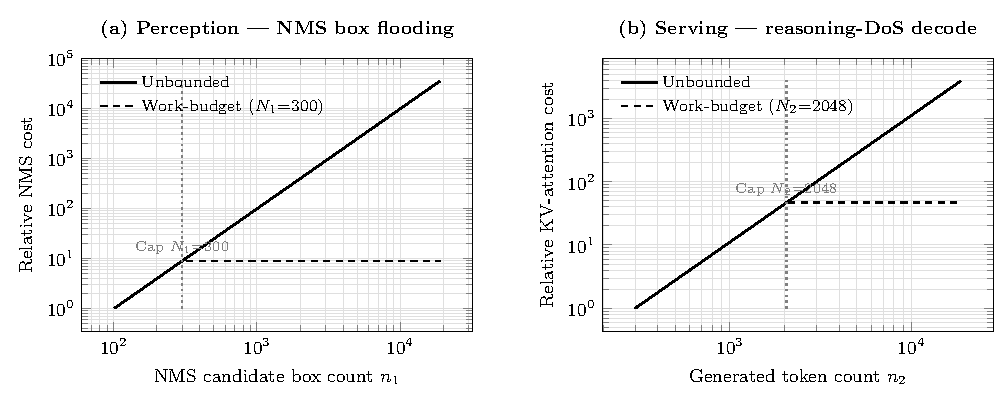
\includegraphics[width=\textwidth]{figure3_workbudget}  % compiled standalone PDF
  %\caption{The work-budget principle converts an unbounded adversarial   worst case into a design-time constant. \textbf{(a)}~Perception: naive   non-maximum suppression (NMS) cost grows quadratically as a box-flooding   attack inflates the candidate count from ${\sim}101$ to ${\sim}19{,}000$   (Groundswell on YOLOv5s~\cite{xia2026groundswell}); a cap of $N_1{=}300$ holds   worst-case NMS cost at $\Theta(300^2)$, collapsing the amplification factor   from ${\sim}(19000/101)^2$ to at most $(300/101)^2$. \textbf{(b)}~Serving:   quadratic KV-attention decode cost grows as a reasoning denial-of-service   attack inflates completion tokens from ${\sim}300$ to ${\sim}18{,}759$   (ReasoningBomb~\cite{liu2026reasoningbomb}); a token cap $N_2{=}2048$ bounds cost   at $\Theta(2048^2)$. Both panels use log--log axes; the capped curve   (dashed) plateaus at the vertical cap line while the unbounded curve   (solid) keeps rising. Given caps $\{N_i\}$, end-to-end worst-case latency   is bounded by $\sum_i \Theta(N_i^{p_i})$, independent of the input.} Across both perception and serving systems, limiting the number of intermediate objects admitted to computationally expensive stages prevents adversarial inputs from driving unbounded growth in computation. 
  \caption{Conceptual illustration of the work-budget abstraction across perception and serving systems. Across both perception and serving systems, limiting the number of intermediate objects admitted to computationally expensive stages prevents adversarial inputs from driving unbounded computation growth.
  The left panel illustrates candidate-box capping for NMS (e.g., Groundswell on YOLOv5s~\cite{xia2026groundswell}), while the right panel illustrates token-budget enforcement during autoregressive decoding (e.g., ReasoningBomb~\cite{liu2026reasoningbomb}). Both panels use log--log axes; the capped curve   (dashed) plateaus at the vertical cap line while the unbounded curve (solid) keeps rising.  The figure is conceptual and intended to illustrate the common design principle underlying several existing defenses.}
  \label{fig:workbudget}
\end{figure*}
%\paragraph{The intermediate-work amplification principle is universal, and so is its remedy.} As argued in Section~\ref{sec:unifying}, every attack class derives its leverage from forcing a downstream stage to receive more inputs than it was provisioned for. The natural cross-domain abstraction is therefore a \emph{work budget}: an explicit, enforced limit on the number of intermediate objects, tokens, or attention computations processed per unit time, applied at the boundary between stages. We use work budget as an abstract design principle rather than a concrete algorithm. A work budget limits the number of intermediate objects admitted to any stage whose computational complexity grows super-linearly with that count. Existing mechanisms—including detection caps, constant-time NMS, token limits, and reasoning-budget enforcement—can all be viewed as instantiations of this general principle. The implementation is application dependent, but the underlying objective is shared: explicitly bound worst-case computation instead of relying solely on average-case efficiency. Constant-time NMS~\cite{biton2023timing}, detection caps, token budgets~\cite{chen2026tokenbudget}, and conformal reasoning bounds~\cite{wang2026conformal} are all instances of this single idea expressed in different modalities. Recognizing them as one mechanism suggests that a general work-budget enforcement primitive, parameterized per stage, could provide uniform coverage.
%Figure 3 is a useful conceptual addition that strengthens the paper's central thesis by visually connecting perception and serving defenses under a common work-budget abstraction without overstepping the scope of a survey."

\paragraph{No end-to-end defense exists.} Every documented defense (Table~\ref{tab:defenses}) protects one layer and leaves others exposed. A VLM-equipped autonomous vehicle faces simultaneous latency threats at the camera-to-detector boundary (NMS overload, physical projectors), the tracking layer (SlowTrack-style temporal attacks), the LiDAR and cooperative-fusion stages, and the VLM planner's decoder (verbose images, reflection backdoors). Composing defenses across these layers is technically possible but has not been evaluated end-to-end in any published work---a gap we return to below.

\textbf{Takeaway.} Viewed through this lens, latency attacks are less about individual algorithms than about uncontrolled computational growth. Although different application domains expose different bottlenecks, they repeatedly exhibit the same underlying mechanism. This shared perspective motivates the work-budget abstraction and suggests that future defenses may be designed around controlling computation itself rather than protecting individual models. We believe this perspective shifts the focus of future research from defending individual models toward bounding computation throughout the entire inference pipeline.

%% ===================================================================
\subsection{Evaluation Practices and Benchmarks}
\label{sec:eval}

Progress is hampered by fragmented evaluation. Perception-attack papers use datasets such as MOT17, nuScenes, and KITTI, report wall-clock latency on specific GPUs (frequently an NVIDIA 2080~Ti or a Jetson device), and---in the strongest cases---report system-level outcomes on the Baidu Apollo stack and LGSVL simulator~\cite{ma2024slowtrack}. LLM/VLM-serving evaluations instead use vLLM-style serving benchmarks on models ranging up to Llama-3-70B, and report access capacity, token amplification, or detector-bypass rate~\cite{zhang2025pd3f,liu2026reasoningbomb}. Three deficiencies recur. First, there is \emph{no standardized latency threat model} analogous to the $\ell_p$-ball used for evasion: papers leave attacker access, perturbation/query budget, and the target latency metric unspecified or mutually inconsistent. Second, there is \emph{no agreed success metric}---wall-clock time, FPS, FLOPs, energy, crash rate, and access capacity are used interchangeably, defeating cross-paper comparison. Third, \emph{no benchmark jointly stresses perception and serving} under attack, which is precisely what an end-to-end AD-plus-VLM stack would require. We argue that joint latency/robustness protocols---measuring accuracy and timing \emph{simultaneously} under adversarial load---are a prerequisite for trustworthy comparison, because efficiency and robustness interact non-monotonically (Section~\ref{sec:open}).

%% ================Section 10===========================================
\section{Emerging Surfaces and Open Challenges}
\label{sec:open}

\subsection{NMS-Free Detectors and Moving Bottlenecks}
\label{sec:nmsfree}

A salient shift threatens to invalidate much of the object-detection attack literature: modern detectors increasingly remove NMS. YOLOv10~\cite{wang2024yolov10} and DETR-style models~\cite{carion2020detr} replace NMS with one-to-one matching (Hungarian or dual-label assignment) and lightweight decoder heads, eliminating the quadratic post-processing blowup that Phantom Sponges and Overload exploit. This does not eliminate the threat---it relocates it. Plausible new bottlenecks include: the multi-scale feature-aggregation \emph{neck} (PANet/BiFPN), where high-entropy features can be forced through all pyramid levels; the \emph{dual-label assignment} head, where conflicting one-to-one and one-to-many decisions can stall the score comparator; the \emph{task-aligned} top-$k$ selection, where many near-identical scores maximize sorting work; \emph{deformable attention}, where maximizing sampling-point spread induces non-coalesced memory access; and the \emph{one-to-one matching} itself, where near-uniform assignment costs drive worst-case Hungarian iterations ($O(N^3)$). From a real-time-systems perspective, the matching-deadlock surface is especially compelling because it directly threatens worst-case execution-time (WCET) bounds---a well-defined failure mode in safety-critical scheduling. We highlight this as a concrete, under-explored direction: the persistence of latency threats across an architectural change that was \emph{not} motivated by security.

%% ===================================================================
\subsection{Cross-cutting Open Challenges}

\paragraph{Standardized, system-level benchmarks.} Most attacks report per-component timing in incompatible units; few connect to downstream outcomes. SlowTrack's crash-rate evaluation~\cite{ma2024slowtrack} and CP-FREEZER's testbed~\cite{wang2026cpfreezer} are exceptions. The field needs benchmarks that report \emph{both} timing and safety/serviceability impact on common axes.

\paragraph{Physical realizability.} Projector attacks~\cite{ma2024slowperception,muller2025detstorm} demonstrate multi-second physical delays but require active infrastructure; SlowTrack's physical transfer remains preliminary~\cite{ma2024slowtrack}. The gap between strong digital results and robust physical deployment is wide.

\paragraph{Inference-time compute as a new surface.} Reasoning models and MoE routers~\cite{liu2026reasoningbomb,li2026thinktrap,fei2026misrouter} created entirely new attack classes within a single year. As architectures continue to make compute input-dependent, each such mechanism is a candidate target, and defenses lag behind by construction.

\paragraph{Timing as an oracle.} Black-box timing attacks~\cite{nakai2021timing} show that even opaque deployments leak optimization signals, complicating any defense that assumes the attacker's ignorance.

\paragraph{The efficiency--robustness tradeoff.} Every architectural defense---pruning, sparsity, early exit---trades average-case efficiency for worst-case robustness, and the tradeoff is non-monotone~\cite{hasan2025sensing,telintelo2024skipsponge}. Defenses that bound worst-case cost by construction (budget enforcement, WCET guards) are more promising than those that merely reduce average cost.

\paragraph{Detection fragility.} High detection-bypass rates~\cite{liu2026reasoningbomb} argue that anomaly detection alone is insufficient; enforceable budgets and scheduling must complement it.

\paragraph{End-to-end stack evaluation.} A modern autonomy stack with a VLM planner is simultaneously vulnerable at the camera sensor, NMS,  MOT, LiDAR/cooperative fusion, and the LLM decoder, yet no published work evaluates all of these jointly. Building a simulation environment that injects attack stimuli at each layer and measures \emph{system-level} outcomes---collision rate, mission completion, service availability---is, in our view, the most practically important open engineering problem in this space, and the natural home for the work-budget abstraction discussed in Section~\ref{sec:synthesis}.

\paragraph{Defense non-transfer.} Because perception-side and serving-side defenses operate on incompatible attack surfaces (Section~\ref{sec:synthesis}), a heterogeneous stack must currently compose multiple narrowly scoped defenses. Whether a single unifying primitive---work-budget enforcement at every stage boundary---can subsume them without unacceptable accuracy cost is an open question.

Collectively, these challenges indicate that latency attacks are transitioning from isolated algorithmic curiosities to a fundamental systems-security problem. Addressing them will likely require tighter integration between machine learning, systems, hardware, and real-time computing than current research communities typically consider.

%% ===============Section 11=============================================
\section{Conclusion}
\label{sec:conclusion}

Latency attacks extend the security of deep learning beyond correctness to timeliness and resource availability. What began as NMS overload on a single detector has matured into a cross-cutting threat spanning physical autonomous-driving perception, sponge attacks on accelerators, slowdown attacks on every form of conditional computation, and a rapidly expanding frontier of output-length, verbose-image, and reasoning denial-of-service attacks on LLMs and VLMs. The unifying lesson is that \emph{any} mechanism which makes inference cost input-dependent---post-processing, sparsity, early exit, routing, autoregressive generation, inference-time reasoning---becomes an attack surface the moment efficiency is advertised. Defenses are advancing, with hardware-aware training, input purification, and especially budget-enforcement-by-construction showing the most promise. Still, they remain fragmented and bound by a persistent efficiency--robustness tradeoff. Progress will depend on standardized benchmarks that report timing alongside downstream impact, on threat models that take physical and serving realism seriously, and on defenses that control worst-case computational paths rather than merely lowering the average. As deep learning continues to trade fixed cost for input-adaptive efficiency, the availability axis will only grow in importance. We expect availability-oriented attacks to become a permanent component of adversarial machine learning research rather than a niche topic. As future architectures increasingly expose dynamic computation, understanding worst-case inference behavior will likely become as important as improving average-case efficiency.

%% ===================================================================
\bibliographystyle{ACM-Reference-Format}
\bibliography{references}

%% ===================================================================
\appendix
\section{Catalog of Latency, Energy, and Timing Attacks and Defenses}
\label{sec:appendix}

This appendix provides a structured, citable catalog of the works surveyed, organized by attack stage (inference vs.\ training) and by defenses. Each entry records the target architecture, application domain, attacker setting, and links to the paper and released code where available. %A continuously updated, searchable web version of these tables is maintained as a companion repository at \url{https://github.com/<your-org>/awesome-latency-attacks}. 
A companion website is available here: \url{https://github.com/guzonghua/awesome-latency-attacks/}.
Tables~\ref{tab:cat-inference}--\ref{tab:cat-defenses} mirror that resource.

%\onecolumn
%% AUTO-GENERATED appendix tables (gen_tables.py). Do not edit by hand.
{\footnotesize\setlength{\tabcolsep}{3pt}
\begin{longtable}{p{2.4cm} p{2.2cm} p{2.7cm} p{1.2cm} p{2.1cm} >{\centering\arraybackslash}p{0.7cm} >{\centering\arraybackslash}p{0.7cm}}
\caption{Inference-stage latency, energy, and timing attacks on deep learning. \faFilePdf~links to the paper; \faGithub~links to released code (\ding{55}~= none located).}\label{tab:cat-inference}\\
\toprule
\textbf{Attack} & \textbf{Venue (Year)} & \textbf{Target} & \textbf{Domain} & \textbf{Setting} & \textbf{Paper} & \textbf{Code} \\
\midrule\endfirsthead
\caption[]{Inference-stage latency, energy, and timing attacks on deep learning. \faFilePdf~links to the paper; \faGithub~links to released code (\ding{55}~= none located). (continued)}\\
\toprule
\textbf{Attack} & \textbf{Venue (Year)} & \textbf{Target} & \textbf{Domain} & \textbf{Setting} & \textbf{Paper} & \textbf{Code} \\
\midrule\endhead
\midrule\multicolumn{7}{r}{\footnotesize\itshape continued on next page}\\\endfoot
\bottomrule\endlastfoot
Daedalus & arXiv (2019) & Object detection (NMS) & CV / AD & White box (physical) & \href{https://arxiv.org/abs/1902.02067}{\faFilePdf} & \href{https://github.com/NeuralSec/Daedalus-attack}{\faGithub} \\
\addlinespace[1pt]
Sparsity Attacks & IEEE TCAD (2020) & CNNs & CV & White box & \href{https://arxiv.org/abs/2006.08020}{\faFilePdf} & \ding{55} \\
\addlinespace[1pt]
Tracker Hijacking & ICLR (2020) & Multi-object tracking & AD & White box & \href{https://arxiv.org/abs/1905.11026}{\faFilePdf} & \ding{55} \\
\addlinespace[1pt]
Sponge Examples & EuroS\&P (2021) & Transformers + CNNs & CV \& NLP & Black \& white box & \href{https://arxiv.org/abs/2006.03463}{\faFilePdf} & \href{https://github.com/iliaishacked/sponge_examples}{\faGithub} \\
\addlinespace[1pt]
DeepSloth & ICLR (2021) & Multi-exit CNNs & CV & White box & \href{https://arxiv.org/abs/2010.02432}{\faFilePdf} & \href{https://github.com/Sanghyun-Hong/DeepSloth}{\faGithub} \\
\addlinespace[1pt]
Timing Side-Channel AE & IEICE Trans. (2021) & DNN classifiers (timing oracle) & CV & Black box (timing) & \href{https://doi.org/10.1587/transfun.2020CIP0022}{\faFilePdf} & \ding{55} \\
\addlinespace[1pt]
SpikeAttack & ACM/IEEE DAC (2022) & Spiking neural networks & CV & White box & \href{https://dl.acm.org/doi/pdf/10.1145/3489517.3530443}{\faFilePdf} & \ding{55} \\
\addlinespace[1pt]
NMTSloth & ESEC/FSE (2022) & Decoder-based NMT & NLP & White box & \href{https://arxiv.org/abs/2210.03696v1}{\faFilePdf} & \href{https://github.com/SeekingDream/FSE22_NMTSloth}{\faGithub} \\
\addlinespace[1pt]
LLMEffiChecker & ACM TOSEM (2022) & LLMs & NLP & Black \& white box & \href{https://arxiv.org/abs/2210.03696}{\faFilePdf} & \href{https://github.com/Cap-Ning/LLMEffiChecker}{\faGithub} \\
\addlinespace[1pt]
NICGSlowDown & CVPR (2022) & Decoder-based image captioning & CV & White box & \href{https://arxiv.org/abs/2203.15859}{\faFilePdf} & \href{https://github.com/SeekingDream/CVPR22_NICGSlowDown}{\faGithub} \\
\addlinespace[1pt]
SAME & ACL (2023) & Multi-exit transformers & NLP & White box & \href{https://arxiv.org/abs/2305.12228}{\faFilePdf} & \href{https://github.com/MatthewCYM/SAME}{\faGithub} \\
\addlinespace[1pt]
SlowBERT & ACL Findings (2023) & Multi-exit BERT & NLP & White box & \href{https://aclanthology.org/2023.findings-acl.602/}{\faFilePdf} & \ding{55} \\
\addlinespace[1pt]
No-Skim & arXiv (2023) & Skimming language models & NLP & Black \& white box & \href{https://arxiv.org/abs/2312.09494}{\faFilePdf} & \ding{55} \\
\addlinespace[1pt]
Phantom Sponges & WACV (2023) & Object detection (NMS) & CV / AD & White box & \href{https://arxiv.org/abs/2205.13618}{\faFilePdf} & \href{https://github.com/AvishagS422/PhantomSponges}{\faGithub} \\
\addlinespace[1pt]
SlowLiDAR & CVPR (2023) & 3D LiDAR detection & CV / AD & White box & \href{https://openaccess.thecvf.com/content/CVPR2023/papers/Liu_SlowLiDAR_Increasing_the_Latency_of_LiDAR-Based_Detection_Using_Adversarial_Examples_CVPR_2023_paper.pdf}{\faFilePdf} & \href{https://github.com/WUSTL-CSPL/SlowLiDAR}{\faGithub} \\
\addlinespace[1pt]
WIP Tracker Attack & VehicleSec (2023) & Multi-object tracking & AD & White box (patch) & \href{https://doi.org/10.14722/vehiclesec.2023.23063}{\faFilePdf} & \ding{55} \\
\addlinespace[1pt]
Variable-Time Inference & AISec@CCS (2023) & Object detection (NMS timing) & CV & Black box (timing) & \href{https://doi.org/10.1145/3605764.3623912}{\faFilePdf} & \ding{55} \\
\addlinespace[1pt]
Overload & CVPR (2024) & Object detection (edge) & CV / AD & White box & \href{https://arxiv.org/abs/2304.05370}{\faFilePdf} & \ding{55} \\
\addlinespace[1pt]
Beyond PhantomSponges & ACM WiseML (2024) & Object detection (NMS) & CV / AD & White box & \href{https://doi.org/10.1145/3649403.3656485}{\faFilePdf} & \ding{55} \\
\addlinespace[1pt]
SlowTrack & AAAI (2024) & Camera perception (detect+track) & AD & White box & \href{https://arxiv.org/abs/2312.09520}{\faFilePdf} & \href{https://github.com/eaiers/SlowTrack}{\faGithub} \\
\addlinespace[1pt]
SlowPerception & arXiv (2024) & Camera perception (NMS+MOT) & AD & White box (physical, projector) & \href{https://arxiv.org/abs/2406.05800}{\faFilePdf} & \ding{55} \\
\addlinespace[1pt]
TPA (Time-aware) & Pattern Recognition Letters (2024) & Detection + segmentation & AD & White box & \href{https://doi.org/10.1016/j.patrec.2024.01.010}{\faFilePdf} & \ding{55} \\
\addlinespace[1pt]
Steal Now Attack Later & arXiv (2024) & Object detection & CV & Black box & \href{https://arxiv.org/abs/2404.15881}{\faFilePdf} & \ding{55} \\
\addlinespace[1pt]
Energy Attack (multi-exit) & Info. \& Software Tech. (2024) & Adaptive multi-exit networks & CV & Grey box & \href{https://doi.org/10.1016/j.infsof.2024.107653}{\faFilePdf} & \ding{55} \\
\addlinespace[1pt]
Slowdown Causes (SaTML) & IEEE SaTML (2024) & Language models & NLP & White box & \href{https://arxiv.org/abs/2305.18926}{\faFilePdf} & \ding{55} \\
\addlinespace[1pt]
Engorgio & arXiv (2024) & LLMs (output inflation) & NLP & White box + transfer & \href{https://arxiv.org/abs/2412.19394}{\faFilePdf} & \ding{55} \\
\addlinespace[1pt]
Verbose Images & ICLR (2024) & Large VLMs & CV+NLP & White box & \href{https://arxiv.org/abs/2401.11170}{\faFilePdf} & \href{https://github.com/KuofengGao/Verbose_Images}{\faGithub} \\
\addlinespace[1pt]
Uniform Inputs & IEEE SPW (2024) & CNNs (sparsity) & CV & Black box & \href{https://arxiv.org/abs/2403.18587}{\faFilePdf} & \href{https://github.com/and-mill/2024-sponge-example-analysis}{\faGithub} \\
\addlinespace[1pt]
DetStorm & IEEE S\&P (2025) & Camera perception & AD & White box (physical) & \href{https://doi.org/10.1109/SP61157.2025.00236}{\faFilePdf} & \ding{55} \\
\addlinespace[1pt]
Inference-Time Impact Analysis & arXiv (2025) & Full perception (sim.) & AD & Simulation & \href{https://arxiv.org/abs/2505.03850}{\faFilePdf} & \ding{55} \\
\addlinespace[1pt]
DDLS Efficiency Attacks & arXiv (2025) & Early-exit / token-pruning / MoE & CV \& NLP & White \& black box & \href{https://arxiv.org/abs/2506.17621}{\faFilePdf} & \ding{55} \\
\addlinespace[1pt]
TTSlow & IEEE TASLP (2025) & Auto-regressive TTS & Speech & White box & \href{https://arxiv.org/abs/2407.01927}{\faFilePdf} & \ding{55} \\
\addlinespace[1pt]
Crabs & ACL Findings (2025) & LLMs (DoS) & NLP & Black box & \href{https://arxiv.org/abs/2412.13879}{\faFilePdf} & \ding{55} \\
\addlinespace[1pt]
VLMInferSlow & ACL (2025) & VLMs-as-a-service & CV+NLP & Black box & \href{https://aclanthology.org/2025.acl-long.encyclopedia/}{\faFilePdf} & \ding{55} \\
\addlinespace[1pt]
Verbose-Text Induction & arXiv (2025) & VLMs & CV+NLP & White box & \href{https://arxiv.org/abs/2511.16163}{\faFilePdf} & \ding{55} \\
\addlinespace[1pt]
LingoLoop & arXiv (2025) & Multimodal LLMs & CV+NLP & White box & \href{https://arxiv.org/abs/2506.14493}{\faFilePdf} & \ding{55} \\
\addlinespace[1pt]
Bit-Flip NMS Attack & WACV (2025) & Object detection (parameters) & CV / AD & Hardware (Rowhammer) & \href{https://doi.org/10.1109/WACV61041.2025.00653}{\faFilePdf} & \ding{55} \\
\addlinespace[1pt]
Timestep-Compressed Attack & AAAI (2025) & Spiking neural networks & CV & White box & \href{https://arxiv.org/abs/2508.13812}{\faFilePdf} & \ding{55} \\
\addlinespace[1pt]
CP-FREEZER & AAAI (2026) & Cooperative perception (V2V) & AD & White box (testbed) & \href{https://ojs.aaai.org/index.php/AAAI/article/download/37082/41044}{\faFilePdf} & \ding{55} \\
\addlinespace[1pt]
Trajectory-Aware Attack & IEEE TMM (2026) & Multi-object tracking & AD & White box & \href{https://doi.org/10.1109/TMM.2026.3651102}{\faFilePdf} & \ding{55} \\
\addlinespace[1pt]
SPLAT & IEEE TCAD (2026) & Multi-exit dynamic networks & CV & Black box & \href{https://doi.org/10.1109/TCAD.2025.3576320}{\faFilePdf} & \ding{55} \\
\addlinespace[1pt]
RouteHijack & arXiv (2026) & Mixture-of-experts LLMs & NLP & White box & \href{https://arxiv.org/abs/2605.02946}{\faFilePdf} & \ding{55} \\
\addlinespace[1pt]
Misrouter & arXiv (2026) & Mixture-of-experts LLMs & NLP & Black box (input-only) & \href{https://arxiv.org/abs/2605.04446}{\faFilePdf} & \ding{55} \\
\addlinespace[1pt]
ReasoningBomb & ACM CCS (2026) & Large reasoning models & NLP & Black box & \href{https://arxiv.org/abs/2602.00154}{\faFilePdf} & \ding{55} \\
\addlinespace[1pt]
ThinkTrap & NDSS (2026) & Reasoning LLM APIs & NLP & Black box & \href{https://www.ndss-symposium.org/ndss2026/}{\faFilePdf} & \ding{55} \\
\addlinespace[1pt]
\end{longtable}}

{\footnotesize\setlength{\tabcolsep}{3pt}
\begin{longtable}{p{2.4cm} p{2.2cm} p{2.7cm} p{1.2cm} p{2.1cm} >{\centering\arraybackslash}p{0.7cm} >{\centering\arraybackslash}p{0.7cm}}
\caption{Training-stage (poisoning / backdoor / weight) latency and energy attacks.}\label{tab:cat-training}\\
\toprule
\textbf{Attack} & \textbf{Venue (Year)} & \textbf{Target} & \textbf{Domain} & \textbf{Setting} & \textbf{Paper} & \textbf{Code} \\
\midrule\endfirsthead
\caption[]{Training-stage (poisoning / backdoor / weight) latency and energy attacks. (continued)}\\
\toprule
\textbf{Attack} & \textbf{Venue (Year)} & \textbf{Target} & \textbf{Domain} & \textbf{Setting} & \textbf{Paper} & \textbf{Code} \\
\midrule\endhead
\midrule\multicolumn{7}{r}{\footnotesize\itshape continued on next page}\\\endfoot
\bottomrule\endlastfoot
Sponge Poisoning & arXiv / AsiaCCS (2022) & CNNs & CV & Partial control & \href{https://arxiv.org/abs/2203.08147}{\faFilePdf} & \href{https://github.com/Cinofix/sponge_poisoning_energy_latency_attack}{\faGithub} \\
\addlinespace[1pt]
On-Device Sponge Poisoning & ACM SecTL (2023) & On-device DNNs & CV & Partial control & \href{https://doi.org/10.1145/3591197.3591307}{\faFilePdf} & \ding{55} \\
\addlinespace[1pt]
Mobile-App Sponge & ACM HotMobile (2023) & Mobile ML models & CV & Partial control & \href{https://doi.org/10.1145/3572864.3581586}{\faFilePdf} & \ding{55} \\
\addlinespace[1pt]
SkipSponge & arXiv (2024) & CNNs, GANs (weights) & CV & Full control & \href{https://arxiv.org/abs/2402.06357}{\faFilePdf} & \ding{55} \\
\addlinespace[1pt]
Huang et al. (multi-exit) & IEEE Access (2024) & Multi-exit CNNs & CV & Full control & \href{https://doi.org/10.1109/ACCESS.2024.3370849}{\faFilePdf} & \ding{55} \\
\addlinespace[1pt]
Sponge Backdoor (OD) & IJCNN (2024) & Object detection (NMS) & CV / AD & Backdoor & \href{https://doi.org/10.1109/IJCNN60899.2024.10650435}{\faFilePdf} & \ding{55} \\
\addlinespace[1pt]
DoS Poisoning (LLM) & arXiv (2024) & LLMs (no-EOS) & NLP & Backdoor / poisoning & \href{https://arxiv.org/abs/2410.10760}{\faFilePdf} & \ding{55} \\
\addlinespace[1pt]
Sensing-AI Sponge & IEEE GLOBECOM (2025) & Sensing DNNs (IoT) & Sensing & Partial control & \href{https://doi.org/10.1109/GLOBECOM59602.2025.11432163}{\faFilePdf} & \ding{55} \\
\addlinespace[1pt]
EvoWeight (FPGA) & IEEE HOST (2025) & FPGA DNN accelerators & CV & Full control & \href{https://doi.org/10.1109/HOST64725.2025.11050058}{\faFilePdf} & \ding{55} \\
\addlinespace[1pt]
Reflection Backdoor (VLM-AD) & arXiv (2025) & Driving VLM planner & AD & Backdoor (physical trigger) & \href{https://arxiv.org/abs/2505.06413}{\faFilePdf} & \ding{55} \\
\addlinespace[1pt]
\end{longtable}}

{\footnotesize\setlength{\tabcolsep}{3pt}
\begin{longtable}{p{2.4cm} p{2.1cm} p{2.5cm} p{2.4cm} p{1.2cm} >{\centering\arraybackslash}p{0.7cm} >{\centering\arraybackslash}p{0.7cm}}
\caption{Defenses against latency, energy, and timing attacks, by control mechanism.}\label{tab:cat-defenses}\\
\toprule
\textbf{Defense} & \textbf{Venue (Year)} & \textbf{Target} & \textbf{Mechanism} & \textbf{Domain} & \textbf{Paper} & \textbf{Code} \\
\midrule\endfirsthead
\caption[]{Defenses against latency, energy, and timing attacks, by control mechanism. (continued)}\\
\toprule
\textbf{Defense} & \textbf{Venue (Year)} & \textbf{Target} & \textbf{Mechanism} & \textbf{Domain} & \textbf{Paper} & \textbf{Code} \\
\midrule\endhead
\midrule\multicolumn{7}{r}{\footnotesize\itshape continued on next page}\\\endfoot
\bottomrule\endlastfoot
DEE Scheduling & ACM CIKM (2021) & Early-exit networks & Runtime scheduling & CV & \href{https://doi.org/10.1145/3459637.3482335}{\faFilePdf} & \ding{55} \\
\addlinespace[1pt]
Certifier Caveat & arXiv (2021) & Certified classifiers & Defense pitfall & CV & \href{https://arxiv.org/abs/2108.11299}{\faFilePdf} & \ding{55} \\
\addlinespace[1pt]
Constant-Time NMS & AISec@CCS (2023) & Object detection (NMS) & Bounded execution & CV & \href{https://doi.org/10.1145/3605764.3623912}{\faFilePdf} & \ding{55} \\
\addlinespace[1pt]
PSML & arXiv (2023) & Inference serving systems & System / serving control & ML serving & \href{https://arxiv.org/abs/2307.01292}{\faFilePdf} & \ding{55} \\
\addlinespace[1pt]
Adaptive Resizing & ACM WiseML (2024) & Object detection (NMS) & Input transformation & AD & \href{https://doi.org/10.1145/3649403.3656485}{\faFilePdf} & \ding{55} \\
\addlinespace[1pt]
ADAV Patch Defense & arXiv (2024) & Object detection & Input transformation & AD & \href{https://arxiv.org/abs/2412.06215}{\faFilePdf} & \ding{55} \\
\addlinespace[1pt]
Securing AV Perception & IEEE TIV (2024) & AV visual perception & Input transformation & AD & \href{https://doi.org/10.1109/TIV.2024.3403667}{\faFilePdf} & \ding{55} \\
\addlinespace[1pt]
Calibration Defense & IEEE SaTML (2024) & Multi-exit models & Robust training & NLP & \href{https://arxiv.org/abs/2305.18926}{\faFilePdf} & \ding{55} \\
\addlinespace[1pt]
Sparsity Monitor & IEEE SPW (2024) & CNNs & Runtime monitoring & CV & \href{https://arxiv.org/abs/2403.18587}{\faFilePdf} & \href{https://github.com/and-mill/2024-sponge-example-analysis}{\faGithub} \\
\addlinespace[1pt]
Garrison & ACM/IEEE DAC (2024) & Ensemble inference (GPU) & System / serving control & CV & \href{https://doi.org/10.1145/3649329.3654810}{\faFilePdf} & \ding{55} \\
\addlinespace[1pt]
Time-Traveling Defense & arXiv (2024) & Traffic-sign classifiers & Temporal redundancy & AD & \href{https://arxiv.org/abs/2410.08338}{\faFilePdf} & \ding{55} \\
\addlinespace[1pt]
Can't Slow Me Down & CVPR (2025) & Edge object detectors & Robust/adaptive training & AD & \href{https://doi.org/10.1109/CVPR52734.2025.01791}{\faFilePdf} & \ding{55} \\
\addlinespace[1pt]
DCT Patch Elimination & IEEE RCAR (2025) & Object detection & Input transformation & AD & \href{https://doi.org/10.1109/RCAR65431.2025.11139457}{\faFilePdf} & \ding{55} \\
\addlinespace[1pt]
Real-Time LiDAR Defense & ACM CCS (2025) & LiDAR detection & Runtime monitoring & AD & \href{https://doi.org/10.1145/3719027.3765227}{\faFilePdf} & \ding{55} \\
\addlinespace[1pt]
LDP Purification & IEEE TrustCom (2025) & VLM visual encoders & Input purification & CV+NLP & \href{https://doi.org/10.1109/Trustcom66490.2025.00065}{\faFilePdf} & \ding{55} \\
\addlinespace[1pt]
Pruning Defense & IEEE GLOBECOM (2025) & Sensing DNNs & Architectural sparsity & Sensing & \href{https://doi.org/10.1109/GLOBECOM59602.2025.11432163}{\faFilePdf} & \ding{55} \\
\addlinespace[1pt]
BlindSight & arXiv (2025) & VLMs & Architectural sparsity & CV+NLP & \href{https://arxiv.org/abs/2507.09071}{\faFilePdf} & \ding{55} \\
\addlinespace[1pt]
PD3F & EMNLP (2025) & LLM serving & Budget enforcement & NLP & \href{https://arxiv.org/abs/2505.18680}{\faFilePdf} & \ding{55} \\
\addlinespace[1pt]
SQUAD & arXiv (2026) & Early-exit ensembles & Runtime scheduling & CV & \href{https://arxiv.org/abs/2601.22711}{\faFilePdf} & \ding{55} \\
\addlinespace[1pt]
Token-Budget Routing & arXiv (2026) & LLM serving & Budget enforcement & NLP & \ding{55} & \ding{55} \\
\addlinespace[1pt]
Conformal Thinking & arXiv (2026) & Reasoning models & Budget enforcement & NLP & \href{https://arxiv.org/abs/2602.03814}{\faFilePdf} & \ding{55} \\
\addlinespace[1pt]
\end{longtable}}

%\twocolumn

\end{document}
